\section{Varying Nodes}
In this chapter we observe what happens when the number of nodes in the system varies. We summarize the value of coverage percentage and the coverage time in the table below.
\begin{table}[h!]
\centering
\resizebox{\textwidth}{!}{%
\begin{tabular}{|l|l|llllll|llllll|}
\hline
                            &                             & \multicolumn{6}{c|}{Coverage percentage}                                                                                                                                                                                                                                                                                 & \multicolumn{6}{c|}{Coverage time}                                                                                                                                                                                                                                                                                       \\ \hline
r                           & n                           & \multicolumn{1}{l|}{p=0,15}                           & \multicolumn{1}{l|}{p=0,3}                            & \multicolumn{1}{l|}{p=0,5}                            & \multicolumn{1}{l|}{p=0,7}                            & \multicolumn{1}{l|}{p=0,85}                           & p=1                              & \multicolumn{1}{l|}{p=0,15}                           & \multicolumn{1}{l|}{p=0,3}                            & \multicolumn{1}{l|}{p=0,5}                            & \multicolumn{1}{l|}{p=0,7}                            & \multicolumn{1}{l|}{p=0,85}                           & p=1                              \\ \hline
\cellcolor[HTML]{5A8AC6}10  & \cellcolor[HTML]{5A8AC6}50  & \multicolumn{1}{l|}{\cellcolor[HTML]{F86A6B}0,024482} & \multicolumn{1}{l|}{\cellcolor[HTML]{F86A6B}0,024482} & \multicolumn{1}{l|}{\cellcolor[HTML]{F86A6B}0,024482} & \multicolumn{1}{l|}{\cellcolor[HTML]{F86A6B}0,025843} & \multicolumn{1}{l|}{\cellcolor[HTML]{F86A6B}0,025665} & \cellcolor[HTML]{F86A6B}0,025665 & \multicolumn{1}{l|}{\cellcolor[HTML]{FCFCFF}17,16667} & \multicolumn{1}{l|}{\cellcolor[HTML]{93B2DA}6,984848} & \multicolumn{1}{l|}{\cellcolor[HTML]{7AA0D1}4,560606} & \multicolumn{1}{l|}{\cellcolor[HTML]{6E98CD}3,469697} & \multicolumn{1}{l|}{\cellcolor[HTML]{FCFCFF}17,16667} & \cellcolor[HTML]{6692CA}2,651515 \\ \hline
\cellcolor[HTML]{5A8AC6}10  & \cellcolor[HTML]{90B0D9}100 & \multicolumn{1}{l|}{\cellcolor[HTML]{F8696B}0,02159}  & \multicolumn{1}{l|}{\cellcolor[HTML]{F86A6B}0,024533} & \multicolumn{1}{l|}{\cellcolor[HTML]{F8696B}0,017109} & \multicolumn{1}{l|}{\cellcolor[HTML]{F8696B}0,016526} & \multicolumn{1}{l|}{\cellcolor[HTML]{F8696B}0,018371} & \cellcolor[HTML]{F8696B}0,02299  & \multicolumn{1}{l|}{\cellcolor[HTML]{FBD6D9}41,37879} & \multicolumn{1}{l|}{\cellcolor[HTML]{FCF9FC}18,92424} & \multicolumn{1}{l|}{\cellcolor[HTML]{C5D5EB}11,71212} & \multicolumn{1}{l|}{\cellcolor[HTML]{A1BCDF}8,318182} & \multicolumn{1}{l|}{\cellcolor[HTML]{FBD6D9}41,37879} & \cellcolor[HTML]{80A5D3}5,166667 \\ \hline
\cellcolor[HTML]{5A8AC6}10  & \cellcolor[HTML]{FCFCFF}200 & \multicolumn{1}{l|}{\cellcolor[HTML]{FDCF7E}0,747209} & \multicolumn{1}{l|}{\cellcolor[HTML]{FDD37F}0,7723}   & \multicolumn{1}{l|}{\cellcolor[HTML]{FCB97A}0,588076} & \multicolumn{1}{l|}{\cellcolor[HTML]{FBA877}0,468021} & \multicolumn{1}{l|}{\cellcolor[HTML]{FA9172}0,304903} & \cellcolor[HTML]{F9826F}0,197414 & \multicolumn{1}{l|}{\cellcolor[HTML]{F8696B}111,0152} & \multicolumn{1}{l|}{\cellcolor[HTML]{FBB6B9}61,86364} & \multicolumn{1}{l|}{\cellcolor[HTML]{FCDCDF}37,83333} & \multicolumn{1}{l|}{\cellcolor[HTML]{FCEBEE}28,01515} & \multicolumn{1}{l|}{\cellcolor[HTML]{F8696B}111,0152} & \cellcolor[HTML]{FCFCFF}16,89394 \\ \hline
\cellcolor[HTML]{5A8AC6}10  & \cellcolor[HTML]{FAA4A7}500 & \multicolumn{1}{l|}{\cellcolor[HTML]{68C07C}0,998189} & \multicolumn{1}{l|}{\cellcolor[HTML]{73C37C}0,994068} & \multicolumn{1}{l|}{\cellcolor[HTML]{9BCE7F}0,978308} & \multicolumn{1}{l|}{\cellcolor[HTML]{EEE784}0,945551} & \multicolumn{1}{l|}{\cellcolor[HTML]{FEE683}0,906997} & \cellcolor[HTML]{FEDC81}0,83855  & \multicolumn{1}{l|}{\cellcolor[HTML]{FAB0B3}65,62121} & \multicolumn{1}{l|}{\cellcolor[HTML]{FCDADD}38,89394} & \multicolumn{1}{l|}{\cellcolor[HTML]{FCEAED}28,43939} & \multicolumn{1}{l|}{\cellcolor[HTML]{FCF0F3}24,92424} & \multicolumn{1}{l|}{\cellcolor[HTML]{FAB0B3}65,62121} & \cellcolor[HTML]{FCF6F9}21,07576 \\ \hline
\cellcolor[HTML]{5A8AC6}10  & \cellcolor[HTML]{F8696B}700 & \multicolumn{1}{l|}{\cellcolor[HTML]{65BF7C}0,999567} & \multicolumn{1}{l|}{\cellcolor[HTML]{6DC17C}0,996217} & \multicolumn{1}{l|}{\cellcolor[HTML]{94CC7E}0,98109}  & \multicolumn{1}{l|}{\cellcolor[HTML]{C1D981}0,963497} & \multicolumn{1}{l|}{\cellcolor[HTML]{FEEA83}0,93384}  & \cellcolor[HTML]{FEE182}0,874377 & \multicolumn{1}{l|}{\cellcolor[HTML]{FBB6B9}62,01515} & \multicolumn{1}{l|}{\cellcolor[HTML]{FCDCDF}37,80303} & \multicolumn{1}{l|}{\cellcolor[HTML]{FCEBEE}27,95455} & \multicolumn{1}{l|}{\cellcolor[HTML]{FCF1F4}24,4697}  & \multicolumn{1}{l|}{\cellcolor[HTML]{FBB6B9}62,01515} & \cellcolor[HTML]{FCF6F9}21,04545 \\ \hline \hline \hline
\cellcolor[HTML]{ABC3E2}30  & \cellcolor[HTML]{5A8AC6}50  & \multicolumn{1}{l|}{\cellcolor[HTML]{FEE081}0,86282}  & \multicolumn{1}{l|}{\cellcolor[HTML]{9ECF7F}0,977003} & \multicolumn{1}{l|}{\cellcolor[HTML]{FEE983}0,92532}  & \multicolumn{1}{l|}{\cellcolor[HTML]{FEE482}0,89483}  & \multicolumn{1}{l|}{\cellcolor[HTML]{FDCF7E}0,74599}  & \cellcolor[HTML]{FBAD78}0,500591 & \multicolumn{1}{l|}{\cellcolor[HTML]{FCE2E5}33,71212} & \multicolumn{1}{l|}{\cellcolor[HTML]{FCFAFD}18,77273} & \multicolumn{1}{l|}{\cellcolor[HTML]{DDE6F4}13,98485} & \multicolumn{1}{l|}{\cellcolor[HTML]{BACDE7}10,65152} & \multicolumn{1}{l|}{\cellcolor[HTML]{AFC6E4}9,621212} & \cellcolor[HTML]{8EAED8}6,469697 \\ \hline
\cellcolor[HTML]{ABC3E2}30  & \cellcolor[HTML]{90B0D9}100 & \multicolumn{1}{l|}{\cellcolor[HTML]{63BE7B}1}        & \multicolumn{1}{l|}{\cellcolor[HTML]{84C87D}0,98707}  & \multicolumn{1}{l|}{\cellcolor[HTML]{FCEA84}0,940233} & \multicolumn{1}{l|}{\cellcolor[HTML]{FEE783}0,912344} & \multicolumn{1}{l|}{\cellcolor[HTML]{FEDF81}0,854607} & \cellcolor[HTML]{FCB77A}0,574112 & \multicolumn{1}{l|}{\cellcolor[HTML]{FCE0E2}35,37879} & \multicolumn{1}{l|}{\cellcolor[HTML]{FCF3F5}23,25758} & \multicolumn{1}{l|}{\cellcolor[HTML]{F6F7FC}16,34848} & \multicolumn{1}{l|}{\cellcolor[HTML]{DBE5F3}13,80303} & \multicolumn{1}{l|}{\cellcolor[HTML]{C1D2EA}11,28788} & \cellcolor[HTML]{9CB8DD}7,833333 \\ \hline
\cellcolor[HTML]{ABC3E2}30  & \cellcolor[HTML]{FCFCFF}200 & \multicolumn{1}{l|}{\cellcolor[HTML]{63BE7B}1}        & \multicolumn{1}{l|}{\cellcolor[HTML]{6DC17C}0,996414} & \multicolumn{1}{l|}{\cellcolor[HTML]{84C87D}0,987382} & \multicolumn{1}{l|}{\cellcolor[HTML]{D5DF82}0,955466} & \multicolumn{1}{l|}{\cellcolor[HTML]{FEE282}0,881255} & \cellcolor[HTML]{FDC67C}0,677805 & \multicolumn{1}{l|}{\cellcolor[HTML]{FBD0D3}45,13636} & \multicolumn{1}{l|}{\cellcolor[HTML]{FCEEF1}26,01515} & \multicolumn{1}{l|}{\cellcolor[HTML]{FCF7FA}20,56061} & \multicolumn{1}{l|}{\cellcolor[HTML]{FCFCFF}17,19697} & \multicolumn{1}{l|}{\cellcolor[HTML]{DAE4F3}13,68182} & \cellcolor[HTML]{B2C8E5}9,924242 \\ \hline
\cellcolor[HTML]{ABC3E2}30  & \cellcolor[HTML]{FAA4A7}500 & \multicolumn{1}{l|}{\cellcolor[HTML]{63BE7B}1}        & \multicolumn{1}{l|}{\cellcolor[HTML]{66BF7C}0,999182} & \multicolumn{1}{l|}{\cellcolor[HTML]{7DC67D}0,989961} & \multicolumn{1}{l|}{\cellcolor[HTML]{D3DF82}0,956269} & \multicolumn{1}{l|}{\cellcolor[HTML]{FEE783}0,913185} & \cellcolor[HTML]{FDC87D}0,695982 & \multicolumn{1}{l|}{\cellcolor[HTML]{FBBCBE}58,34848} & \multicolumn{1}{l|}{\cellcolor[HTML]{FCD8DB}40,22727} & \multicolumn{1}{l|}{\cellcolor[HTML]{FCE7EA}30,59091} & \multicolumn{1}{l|}{\cellcolor[HTML]{FCF1F4}24,22727} & \multicolumn{1}{l|}{\cellcolor[HTML]{FCF8FB}19,65152} & \cellcolor[HTML]{D4E0F1}13,13636 \\ \hline
\cellcolor[HTML]{ABC3E2}30  & \cellcolor[HTML]{F8696B}700 & \multicolumn{1}{l|}{\cellcolor[HTML]{63BE7B}1}        & \multicolumn{1}{l|}{\cellcolor[HTML]{6AC07C}0,997563} & \multicolumn{1}{l|}{\cellcolor[HTML]{7AC57D}0,990985} & \multicolumn{1}{l|}{\cellcolor[HTML]{BDD881}0,964937} & \multicolumn{1}{l|}{\cellcolor[HTML]{FEEA83}0,935377} & \cellcolor[HTML]{FDCD7E}0,732669 & \multicolumn{1}{l|}{\cellcolor[HTML]{FAB1B4}64,95455} & \multicolumn{1}{l|}{\cellcolor[HTML]{FBD1D3}44,98485} & \multicolumn{1}{l|}{\cellcolor[HTML]{FCE1E4}34,65152} & \multicolumn{1}{l|}{\cellcolor[HTML]{FCEBEE}27,92424} & \multicolumn{1}{l|}{\cellcolor[HTML]{FCF5F8}21,92424} & \cellcolor[HTML]{FCFCFF}16,89394 \\ \hline  \hline \hline
\cellcolor[HTML]{FCFCFF}50  & \cellcolor[HTML]{5A8AC6}50  & \multicolumn{1}{l|}{\cellcolor[HTML]{63BE7B}1}        & \multicolumn{1}{l|}{\cellcolor[HTML]{88C97E}0,985655} & \multicolumn{1}{l|}{\cellcolor[HTML]{FEE783}0,917359} & \multicolumn{1}{l|}{\cellcolor[HTML]{FEE282}0,875088} & \multicolumn{1}{l|}{\cellcolor[HTML]{FED980}0,814974} & \cellcolor[HTML]{FBAD78}0,499584 & \multicolumn{1}{l|}{\cellcolor[HTML]{FCE7EA}30,5303}  & \multicolumn{1}{l|}{\cellcolor[HTML]{F9F9FD}16,62121} & \multicolumn{1}{l|}{\cellcolor[HTML]{CBD9ED}12,28788} & \multicolumn{1}{l|}{\cellcolor[HTML]{AAC2E2}9,136364} & \multicolumn{1}{l|}{\cellcolor[HTML]{97B5DB}7,378788} & \cellcolor[HTML]{6E98CD}3,439394 \\ \hline
\cellcolor[HTML]{FCFCFF}50  & \cellcolor[HTML]{90B0D9}100 & \multicolumn{1}{l|}{\cellcolor[HTML]{63BE7B}1}        & \multicolumn{1}{l|}{\cellcolor[HTML]{69C07C}0,997956} & \multicolumn{1}{l|}{\cellcolor[HTML]{E3E383}0,950017} & \multicolumn{1}{l|}{\cellcolor[HTML]{FEE382}0,888699} & \multicolumn{1}{l|}{\cellcolor[HTML]{FDD27F}0,7652}   & \cellcolor[HTML]{FBA676}0,454022 & \multicolumn{1}{l|}{\cellcolor[HTML]{FCDFE2}35,56061} & \multicolumn{1}{l|}{\cellcolor[HTML]{FCF1F4}24,25758} & \multicolumn{1}{l|}{\cellcolor[HTML]{F7F8FD}16,4697}  & \multicolumn{1}{l|}{\cellcolor[HTML]{CEDCEF}12,59091} & \multicolumn{1}{l|}{\cellcolor[HTML]{A4BEE0}8,560606} & \cellcolor[HTML]{7099CD}3,590909 \\ \hline
\cellcolor[HTML]{FCFCFF}50  & \cellcolor[HTML]{FCFCFF}200 & \multicolumn{1}{l|}{\cellcolor[HTML]{63BE7B}1}        & \multicolumn{1}{l|}{\cellcolor[HTML]{9FD07F}0,976742} & \multicolumn{1}{l|}{\cellcolor[HTML]{F6E984}0,942634} & \multicolumn{1}{l|}{\cellcolor[HTML]{FEE582}0,898068} & \multicolumn{1}{l|}{\cellcolor[HTML]{FDD57F}0,788035} & \cellcolor[HTML]{FBAD78}0,500295 & \multicolumn{1}{l|}{\cellcolor[HTML]{FBCACD}49,04545} & \multicolumn{1}{l|}{\cellcolor[HTML]{FCE9EC}29,59091} & \multicolumn{1}{l|}{\cellcolor[HTML]{FCF6F9}21,31818} & \multicolumn{1}{l|}{\cellcolor[HTML]{EEF2FA}15,65152} & \multicolumn{1}{l|}{\cellcolor[HTML]{BFD1E9}11,10606} & \cellcolor[HTML]{729BCE}3,80303  \\ \hline
\cellcolor[HTML]{FCFCFF}50  & \cellcolor[HTML]{FAA4A7}500 & \multicolumn{1}{l|}{\cellcolor[HTML]{63BE7B}1}        & \multicolumn{1}{l|}{\cellcolor[HTML]{6FC27C}0,995504} & \multicolumn{1}{l|}{\cellcolor[HTML]{89C97E}0,985126} & \multicolumn{1}{l|}{\cellcolor[HTML]{FEE783}0,913678} & \multicolumn{1}{l|}{\cellcolor[HTML]{FDD07E}0,749905} & \cellcolor[HTML]{FBA877}0,463861 & \multicolumn{1}{l|}{\cellcolor[HTML]{FAADB0}67,71212} & \multicolumn{1}{l|}{\cellcolor[HTML]{FBD0D2}45,5303}  & \multicolumn{1}{l|}{\cellcolor[HTML]{FCE7EA}30,5303}  & \multicolumn{1}{l|}{\cellcolor[HTML]{FCF6F9}21,04545} & \multicolumn{1}{l|}{\cellcolor[HTML]{DCE5F3}13,89394} & \cellcolor[HTML]{7DA2D2}4,863636 \\ \hline
\cellcolor[HTML]{FCFCFF}50  & \cellcolor[HTML]{F8696B}700 & \multicolumn{1}{l|}{\cellcolor[HTML]{63BE7B}1}        & \multicolumn{1}{l|}{\cellcolor[HTML]{63BE7B}1}        & \multicolumn{1}{l|}{\cellcolor[HTML]{D1DE82}0,957128} & \multicolumn{1}{l|}{\cellcolor[HTML]{FED980}0,814391} & \multicolumn{1}{l|}{\cellcolor[HTML]{FEDA80}0,824465} & \cellcolor[HTML]{FBA676}0,453678 & \multicolumn{1}{l|}{\cellcolor[HTML]{FA9FA1}77,07576} & \multicolumn{1}{l|}{\cellcolor[HTML]{FBCBCE}48,59091} & \multicolumn{1}{l|}{\cellcolor[HTML]{FCE3E6}33,37879} & \multicolumn{1}{l|}{\cellcolor[HTML]{FCF8FB}19,98485} & \multicolumn{1}{l|}{\cellcolor[HTML]{EDF1F9}15,5}     & \cellcolor[HTML]{80A5D3}5,19697  \\ \hline  \hline \hline
\cellcolor[HTML]{FAB3B5}75  & \cellcolor[HTML]{5A8AC6}50  & \multicolumn{1}{l|}{\cellcolor[HTML]{63BE7B}1}        & \multicolumn{1}{l|}{\cellcolor[HTML]{78C57D}0,991825} & \multicolumn{1}{l|}{\cellcolor[HTML]{E3E383}0,94982}  & \multicolumn{1}{l|}{\cellcolor[HTML]{FED980}0,817595} & \multicolumn{1}{l|}{\cellcolor[HTML]{FEDA80}0,823015} & \cellcolor[HTML]{FCBF7B}0,632061 & \multicolumn{1}{l|}{\cellcolor[HTML]{FCE9EB}29,65152} & \multicolumn{1}{l|}{\cellcolor[HTML]{F2F5FB}16,01515} & \multicolumn{1}{l|}{\cellcolor[HTML]{BCCFE8}10,83333} & \multicolumn{1}{l|}{\cellcolor[HTML]{8DADD7}6,348485} & \multicolumn{1}{l|}{\cellcolor[HTML]{7DA3D2}4,893939} & \cellcolor[HTML]{5A8AC6}1,5      \\ \hline
\cellcolor[HTML]{FAB3B5}75  & \cellcolor[HTML]{90B0D9}100 & \multicolumn{1}{l|}{\cellcolor[HTML]{63BE7B}1}        & \multicolumn{1}{l|}{\cellcolor[HTML]{63BE7B}1}        & \multicolumn{1}{l|}{\cellcolor[HTML]{FEE883}0,921545} & \multicolumn{1}{l|}{\cellcolor[HTML]{FEE582}0,896459} & \multicolumn{1}{l|}{\cellcolor[HTML]{FEDA80}0,819265} & \cellcolor[HTML]{FCC27C}0,649472 & \multicolumn{1}{l|}{\cellcolor[HTML]{FCE0E3}35,25758} & \multicolumn{1}{l|}{\cellcolor[HTML]{FCF4F7}22,40909} & \multicolumn{1}{l|}{\cellcolor[HTML]{D7E2F2}13,40909} & \multicolumn{1}{l|}{\cellcolor[HTML]{AAC2E2}9,106061} & \multicolumn{1}{l|}{\cellcolor[HTML]{89ABD6}5,984848} & \cellcolor[HTML]{5A8AC6}1,5      \\ \hline
\cellcolor[HTML]{FAB3B5}75  & \cellcolor[HTML]{FCFCFF}200 & \multicolumn{1}{l|}{\cellcolor[HTML]{63BE7B}1}        & \multicolumn{1}{l|}{\cellcolor[HTML]{63BE7B}1}        & \multicolumn{1}{l|}{\cellcolor[HTML]{C9DC81}0,96036}  & \multicolumn{1}{l|}{\cellcolor[HTML]{FEDD81}0,844924} & \multicolumn{1}{l|}{\cellcolor[HTML]{FDD880}0,806358} & \cellcolor[HTML]{FCC07B}0,638544 & \multicolumn{1}{l|}{\cellcolor[HTML]{FBCCCF}47,65152} & \multicolumn{1}{l|}{\cellcolor[HTML]{FCEFF2}25,31818} & \multicolumn{1}{l|}{\cellcolor[HTML]{FAFBFE}16,77273} & \multicolumn{1}{l|}{\cellcolor[HTML]{B9CCE7}10,5303}  & \multicolumn{1}{l|}{\cellcolor[HTML]{96B4DB}7,257576} & \cellcolor[HTML]{5A8AC6}1,5      \\ \hline
\cellcolor[HTML]{FAB3B5}75  & \cellcolor[HTML]{FAA4A7}500 & \multicolumn{1}{l|}{\cellcolor[HTML]{63BE7B}1}        & \multicolumn{1}{l|}{\cellcolor[HTML]{A9D380}0,972766} & \multicolumn{1}{l|}{\cellcolor[HTML]{FEE783}0,915629} & \multicolumn{1}{l|}{\cellcolor[HTML]{FEE081}0,863574} & \multicolumn{1}{l|}{\cellcolor[HTML]{FDD17F}0,760205} & \cellcolor[HTML]{FCC07B}0,637793 & \multicolumn{1}{l|}{\cellcolor[HTML]{FBB7BA}61,28788} & \multicolumn{1}{l|}{\cellcolor[HTML]{FCE0E2}35,34848} & \multicolumn{1}{l|}{\cellcolor[HTML]{FCF4F7}22,56061} & \multicolumn{1}{l|}{\cellcolor[HTML]{D6E1F1}13,28788} & \multicolumn{1}{l|}{\cellcolor[HTML]{9EBADE}8,045455} & \cellcolor[HTML]{5A8AC6}1,5      \\ \hline
\cellcolor[HTML]{FAB3B5}75  & \cellcolor[HTML]{F8696B}700 & \multicolumn{1}{l|}{\cellcolor[HTML]{63BE7B}1}        & \multicolumn{1}{l|}{\cellcolor[HTML]{8FCB7E}0,982774} & \multicolumn{1}{l|}{\cellcolor[HTML]{FEE783}0,91658}  & \multicolumn{1}{l|}{\cellcolor[HTML]{FEE683}0,909074} & \multicolumn{1}{l|}{\cellcolor[HTML]{FEDB80}0,828044} & \cellcolor[HTML]{FCC17B}0,642411 & \multicolumn{1}{l|}{\cellcolor[HTML]{FAAFB1}66,68182} & \multicolumn{1}{l|}{\cellcolor[HTML]{FCDCDE}38,01515} & \multicolumn{1}{l|}{\cellcolor[HTML]{FCF2F5}23,37879} & \multicolumn{1}{l|}{\cellcolor[HTML]{E0E8F5}14,25758} & \multicolumn{1}{l|}{\cellcolor[HTML]{AFC6E4}9,621212} & \cellcolor[HTML]{5A8AC6}1,5      \\ \hline  \hline \hline
\cellcolor[HTML]{F8696B}100 & \cellcolor[HTML]{5A8AC6}50  & \multicolumn{1}{l|}{\cellcolor[HTML]{63BE7B}1}        & \multicolumn{1}{l|}{\cellcolor[HTML]{63BE7B}1}        & \multicolumn{1}{l|}{\cellcolor[HTML]{98CE7F}0,979562} & \multicolumn{1}{l|}{\cellcolor[HTML]{CDDD82}0,95875}  & \multicolumn{1}{l|}{\cellcolor[HTML]{F6E984}0,942408} & \cellcolor[HTML]{FEE983}0,926149 & \multicolumn{1}{l|}{\cellcolor[HTML]{FCEAED}28,5}     & \multicolumn{1}{l|}{\cellcolor[HTML]{D5E1F1}13,25758} & \multicolumn{1}{l|}{\cellcolor[HTML]{A0BBDE}8,227273} & \multicolumn{1}{l|}{\cellcolor[HTML]{7EA4D3}5,015152} & \multicolumn{1}{l|}{\cellcolor[HTML]{6D97CC}3,378788} & \cellcolor[HTML]{5A8AC6}1,5      \\ \hline
\cellcolor[HTML]{F8696B}100 & \cellcolor[HTML]{90B0D9}100 & \multicolumn{1}{l|}{\cellcolor[HTML]{63BE7B}1}        & \multicolumn{1}{l|}{\cellcolor[HTML]{98CE7F}0,979562} & \multicolumn{1}{l|}{\cellcolor[HTML]{8BCA7E}0,984599} & \multicolumn{1}{l|}{\cellcolor[HTML]{B2D580}0,96916}  & \multicolumn{1}{l|}{\cellcolor[HTML]{D7E082}0,954525} & \cellcolor[HTML]{FEEA83}0,937334 & \multicolumn{1}{l|}{\cellcolor[HTML]{FCE5E8}31,62121} & \multicolumn{1}{l|}{\cellcolor[HTML]{FCFBFE}17,68182} & \multicolumn{1}{l|}{\cellcolor[HTML]{B2C8E5}9,893939} & \multicolumn{1}{l|}{\cellcolor[HTML]{88AAD6}5,893939} & \multicolumn{1}{l|}{\cellcolor[HTML]{789FD0}4,378788} & \cellcolor[HTML]{5A8AC6}1,5      \\ \hline
\cellcolor[HTML]{F8696B}100 & \cellcolor[HTML]{FCFCFF}200 & \multicolumn{1}{l|}{\cellcolor[HTML]{63BE7B}1}        & \multicolumn{1}{l|}{\cellcolor[HTML]{71C27C}0,99489}  & \multicolumn{1}{l|}{\cellcolor[HTML]{97CD7E}0,979734} & \multicolumn{1}{l|}{\cellcolor[HTML]{B6D680}0,967563} & \multicolumn{1}{l|}{\cellcolor[HTML]{F0E784}0,944922} & \cellcolor[HTML]{FEE983}0,928947 & \multicolumn{1}{l|}{\cellcolor[HTML]{FBD7DA}41,01515} & \multicolumn{1}{l|}{\cellcolor[HTML]{FCFAFD}18,28788} & \multicolumn{1}{l|}{\cellcolor[HTML]{BED0E9}11,04545} & \multicolumn{1}{l|}{\cellcolor[HTML]{94B3DA}7,075758} & \multicolumn{1}{l|}{\cellcolor[HTML]{7BA1D1}4,651515} & \cellcolor[HTML]{5A8AC6}1,5      \\ \hline
\cellcolor[HTML]{F8696B}100 & \cellcolor[HTML]{FAA4A7}500 & \multicolumn{1}{l|}{\cellcolor[HTML]{63BE7B}1}        & \multicolumn{1}{l|}{\cellcolor[HTML]{65BF7C}0,999591} & \multicolumn{1}{l|}{\cellcolor[HTML]{97CD7E}0,979969} & \multicolumn{1}{l|}{\cellcolor[HTML]{BED981}0,964415} & \multicolumn{1}{l|}{\cellcolor[HTML]{CFDD82}0,957983} & \cellcolor[HTML]{FEE983}0,929607 & \multicolumn{1}{l|}{\cellcolor[HTML]{FBCCCF}48,04545} & \multicolumn{1}{l|}{\cellcolor[HTML]{FCF0F3}24,71212} & \multicolumn{1}{l|}{\cellcolor[HTML]{D6E1F1}13,28788} & \multicolumn{1}{l|}{\cellcolor[HTML]{9FBADE}8,106061} & \multicolumn{1}{l|}{\cellcolor[HTML]{86A9D5}5,772727} & \cellcolor[HTML]{5A8AC6}1,5      \\ \hline
\cellcolor[HTML]{F8696B}100 & \cellcolor[HTML]{F8696B}700 & \multicolumn{1}{l|}{\cellcolor[HTML]{66BF7C}0,999124} & \multicolumn{1}{l|}{\cellcolor[HTML]{67C07C}0,99854}  & \multicolumn{1}{l|}{\cellcolor[HTML]{9BCE7F}0,9784}   & \multicolumn{1}{l|}{\cellcolor[HTML]{B7D780}0,967052} & \multicolumn{1}{l|}{\cellcolor[HTML]{D2DE82}0,956693} & \cellcolor[HTML]{FEE983}0,931083 & \multicolumn{1}{l|}{\cellcolor[HTML]{FBCACC}49,43939} & \multicolumn{1}{l|}{\cellcolor[HTML]{FCF0F3}24,71212} & \multicolumn{1}{l|}{\cellcolor[HTML]{D7E2F2}13,43939} & \multicolumn{1}{l|}{\cellcolor[HTML]{ABC3E2}9,227273} & \multicolumn{1}{l|}{\cellcolor[HTML]{82A6D4}5,378788} & \cellcolor[HTML]{5A8AC6}1,5      \\ \hline
\end{tabular}%
}
\caption{Coverage percentage and coverage time for different scenarios}
\label{tab:my-table}
\end{table}

It is interesting to notice that lower radii become better at higher number of nodes regarding coverage percentage, this happens because the area in which the nodes are distributed does not change so the density increases and so does the number of neighbor for each node. 
Another thing to notice is that, for the coverage time, the values increase with the number of nodes, but they do far worse when the sending probability is lower; this divides each rectangle (one for each group of radius) in two triangle, the lower left with the worse times and the upper right with the best ones and, at growing radius, the last one get bigger.
Finally we can see that lower probabilities tent to perform better than higher ones for coverage percentage in spite of coverage time independently from the number of nodes and radius except for the first rows.

\section{50 and 700 cases}
At the edges of the node numbers chosen for our configurations we have 50 and 700. We now want to analyze the performance indixes for 50 and then for 700 nodes, to discover any similarities and/or differences with the case at 200. Note how for the configuration of radius 10 at 700 nodes appears to be a valid configuration but due to the symmetry of the graphs at 200 and 50 nodes it is not shown.

\subsection{Coverage percentage}\label{subsec:CovPerc}
\begin{figure}[H]
\minipage{0.50\linewidth}
  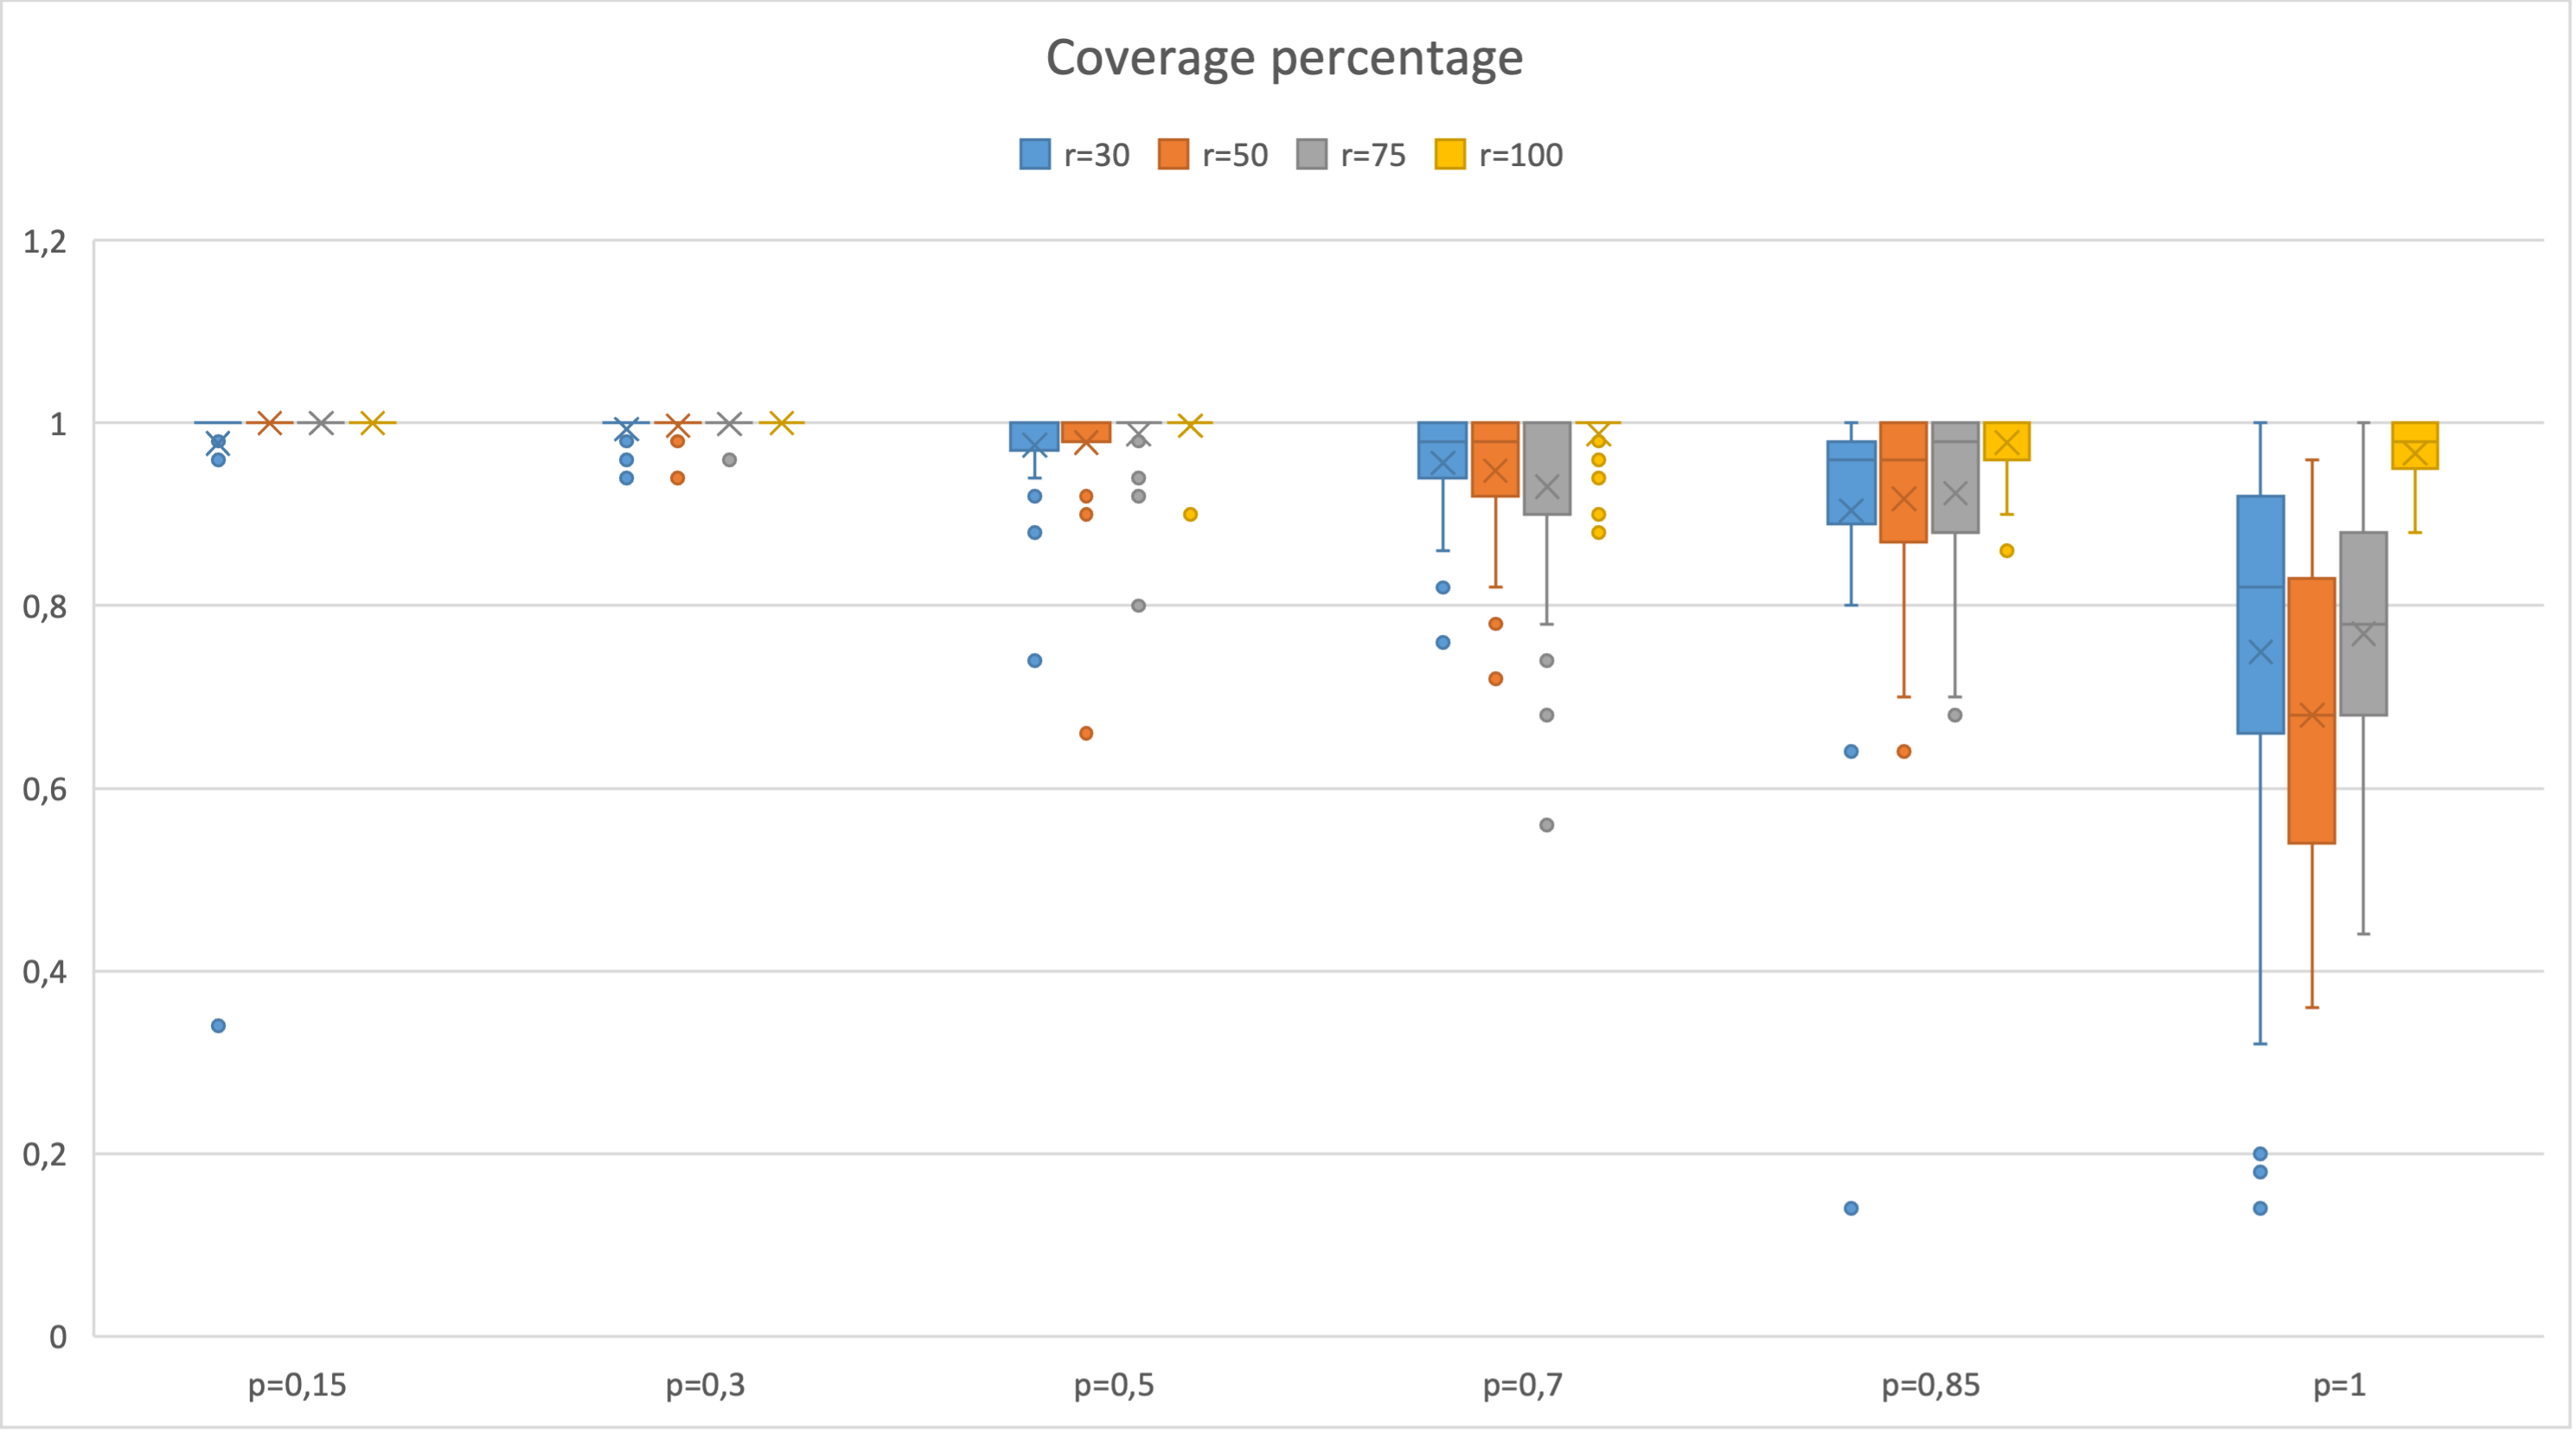
\includegraphics[width=\linewidth]{./images/Rate50Boxplot.png}
  \caption{50 Nodes}\label{fig:awesome_image1}
\endminipage\hfill
\minipage{0.50\linewidth}
  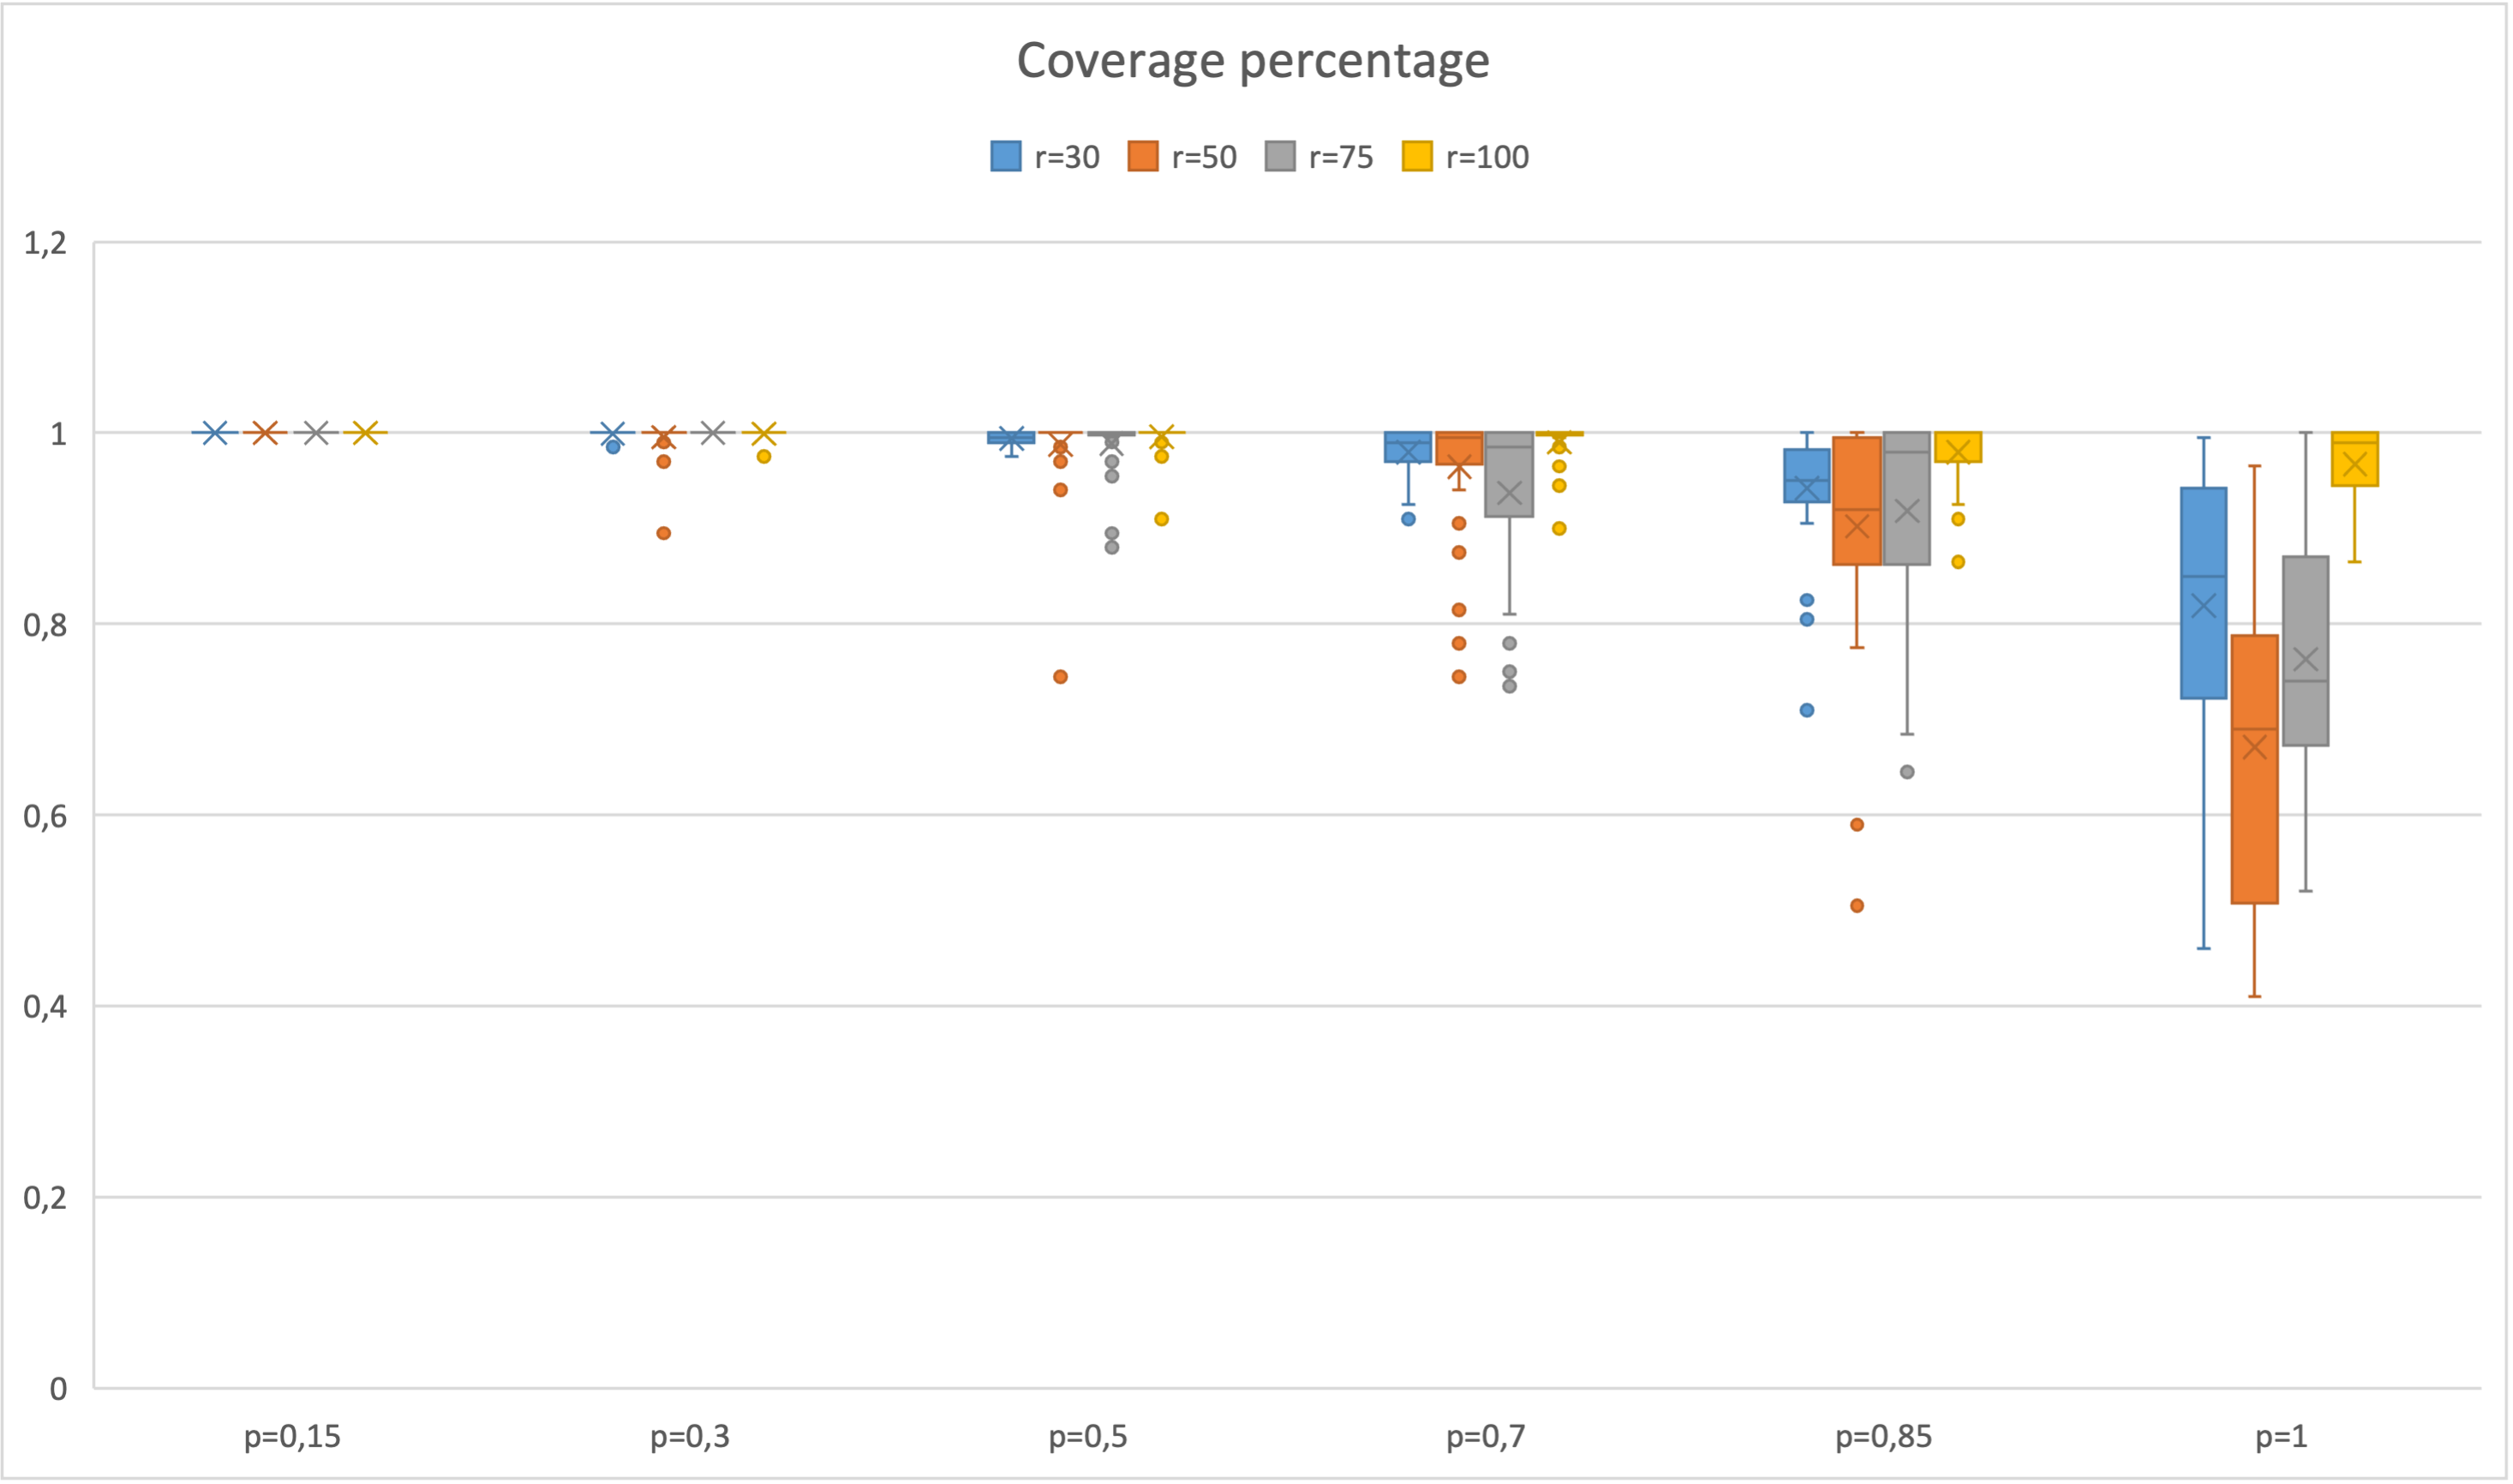
\includegraphics[width=\linewidth]{./images/Rate200Boxplot.png}
  \caption{200 Nodes}\label{fig:awesome_image2}
\endminipage
\end{figure}

\begin{figure}[H]
\minipage{0.50\linewidth}
  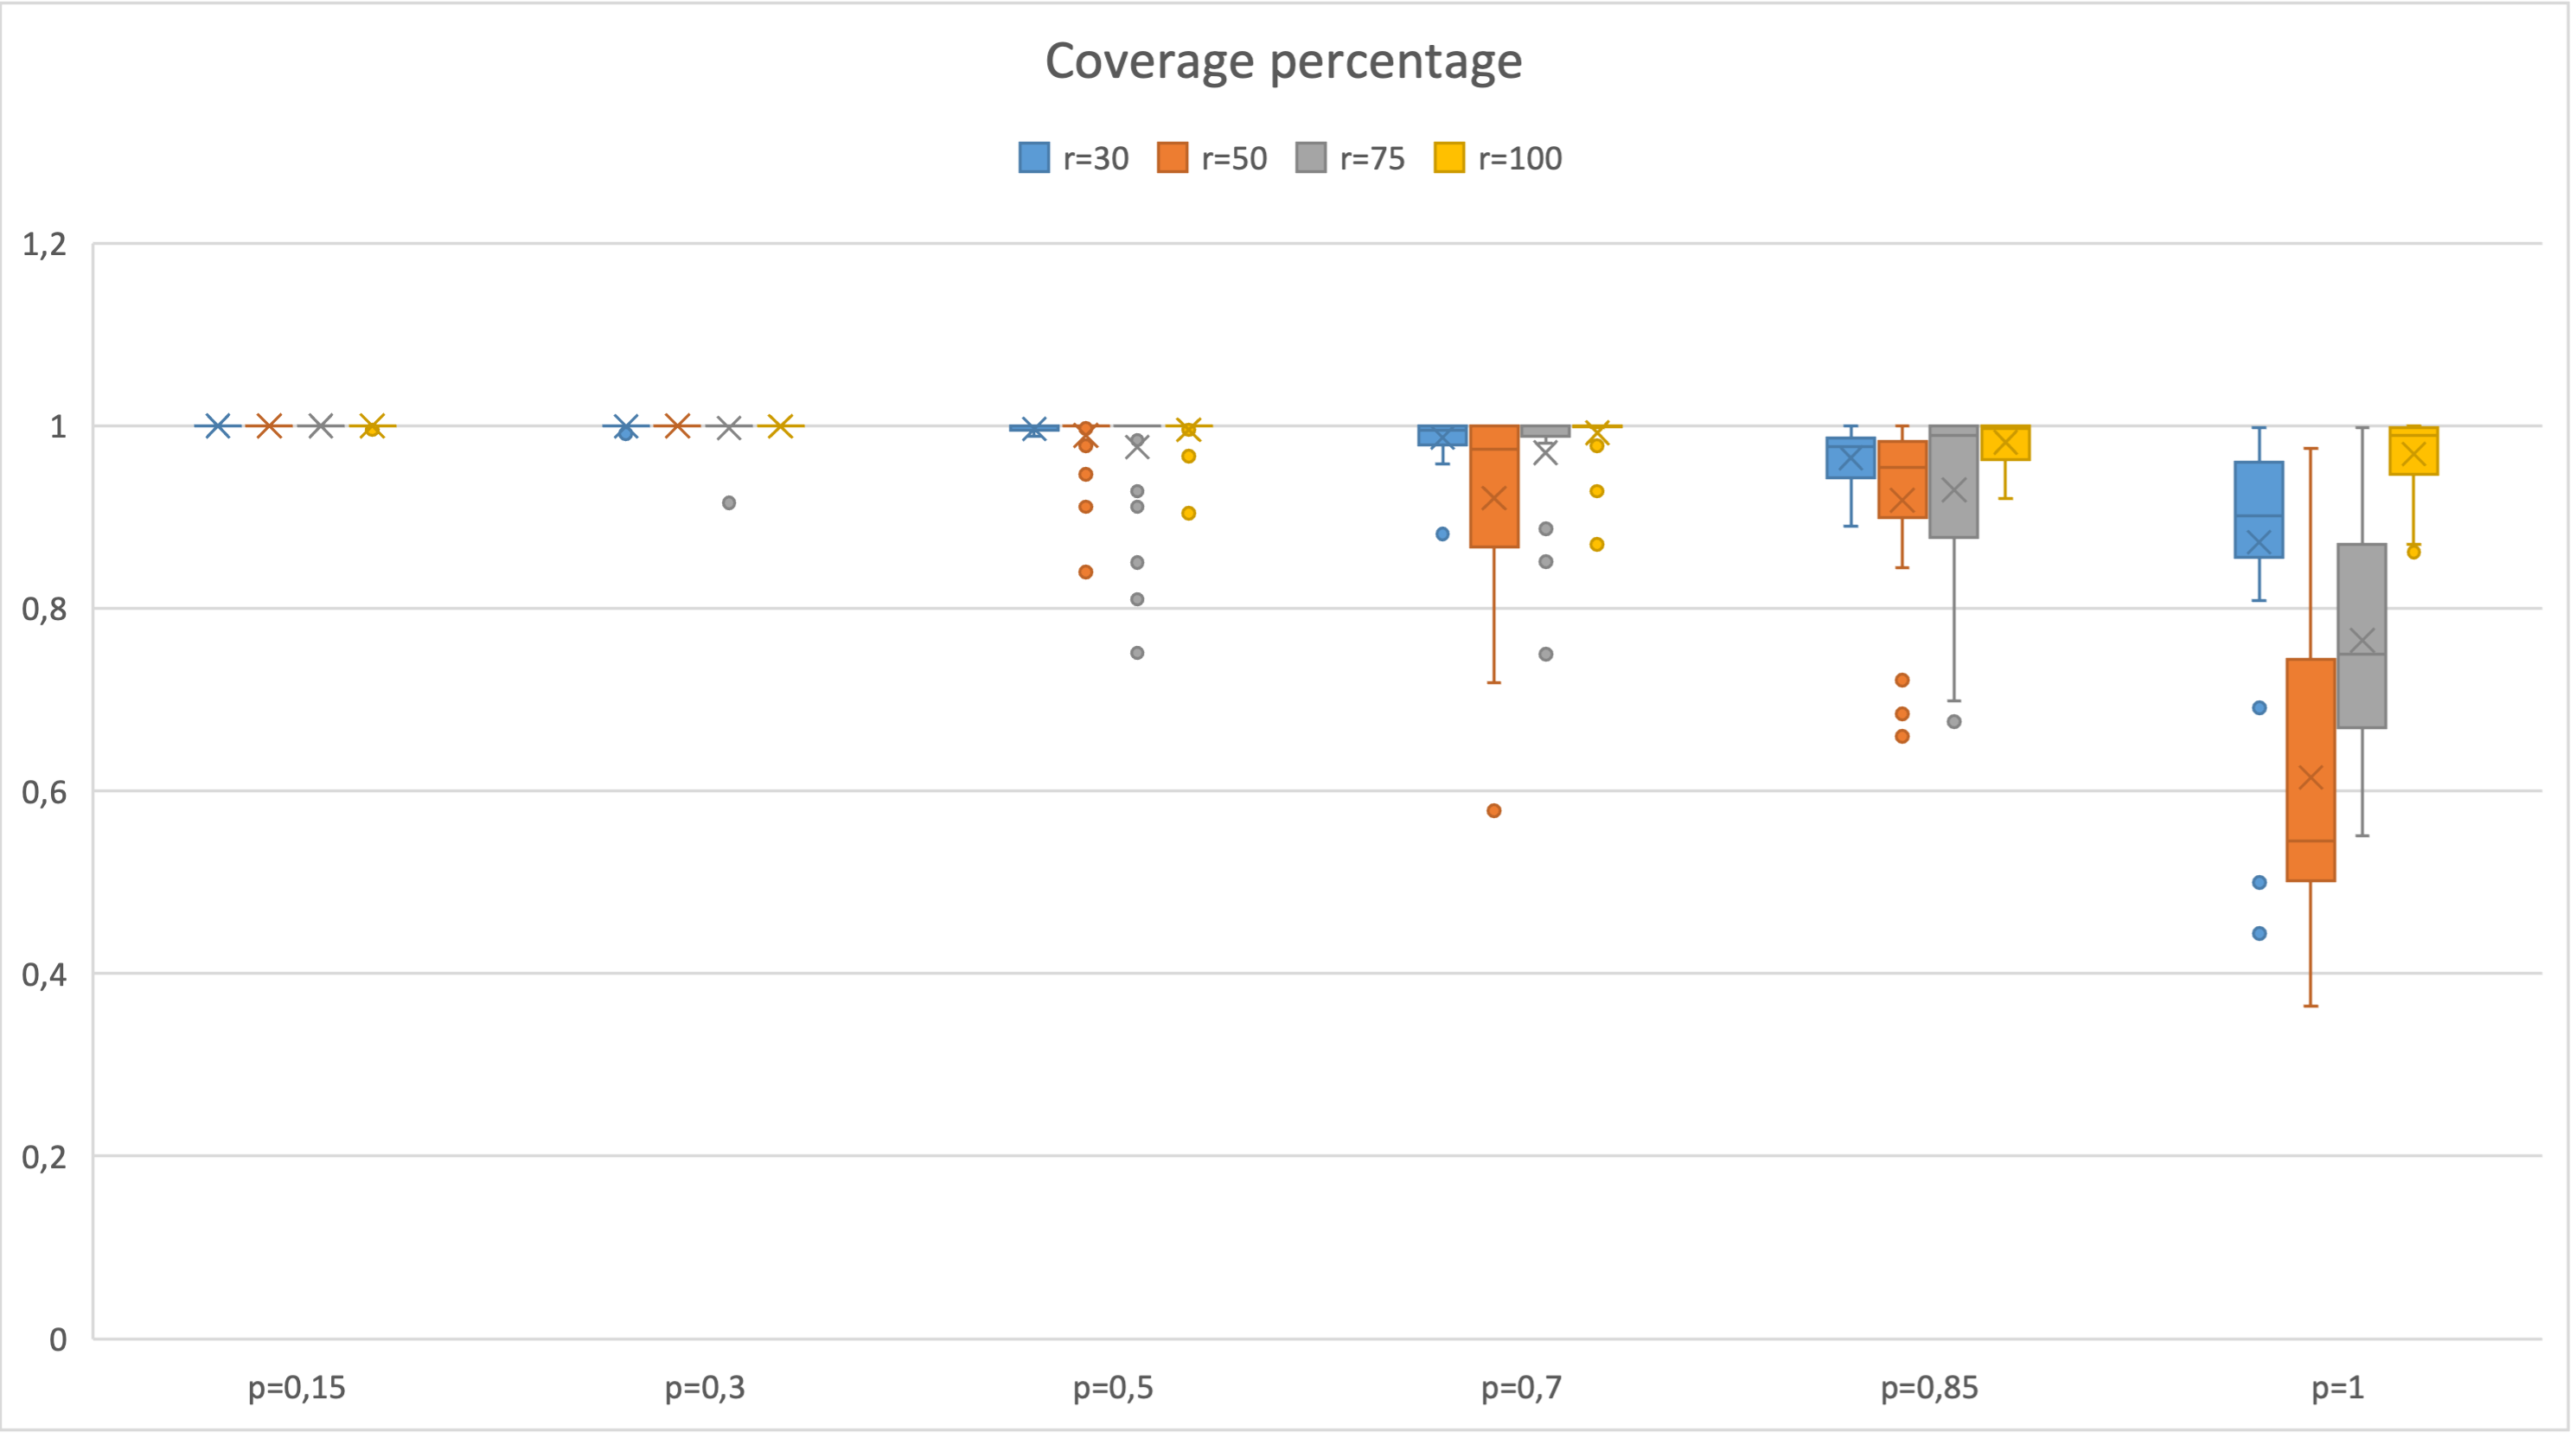
\includegraphics[width=\linewidth]{./images/Rate700Boxplot.png}
  \caption{700 Nodes}\label{fig:awesome_image1}
\endminipage\hfill
\minipage{0.50\linewidth}
  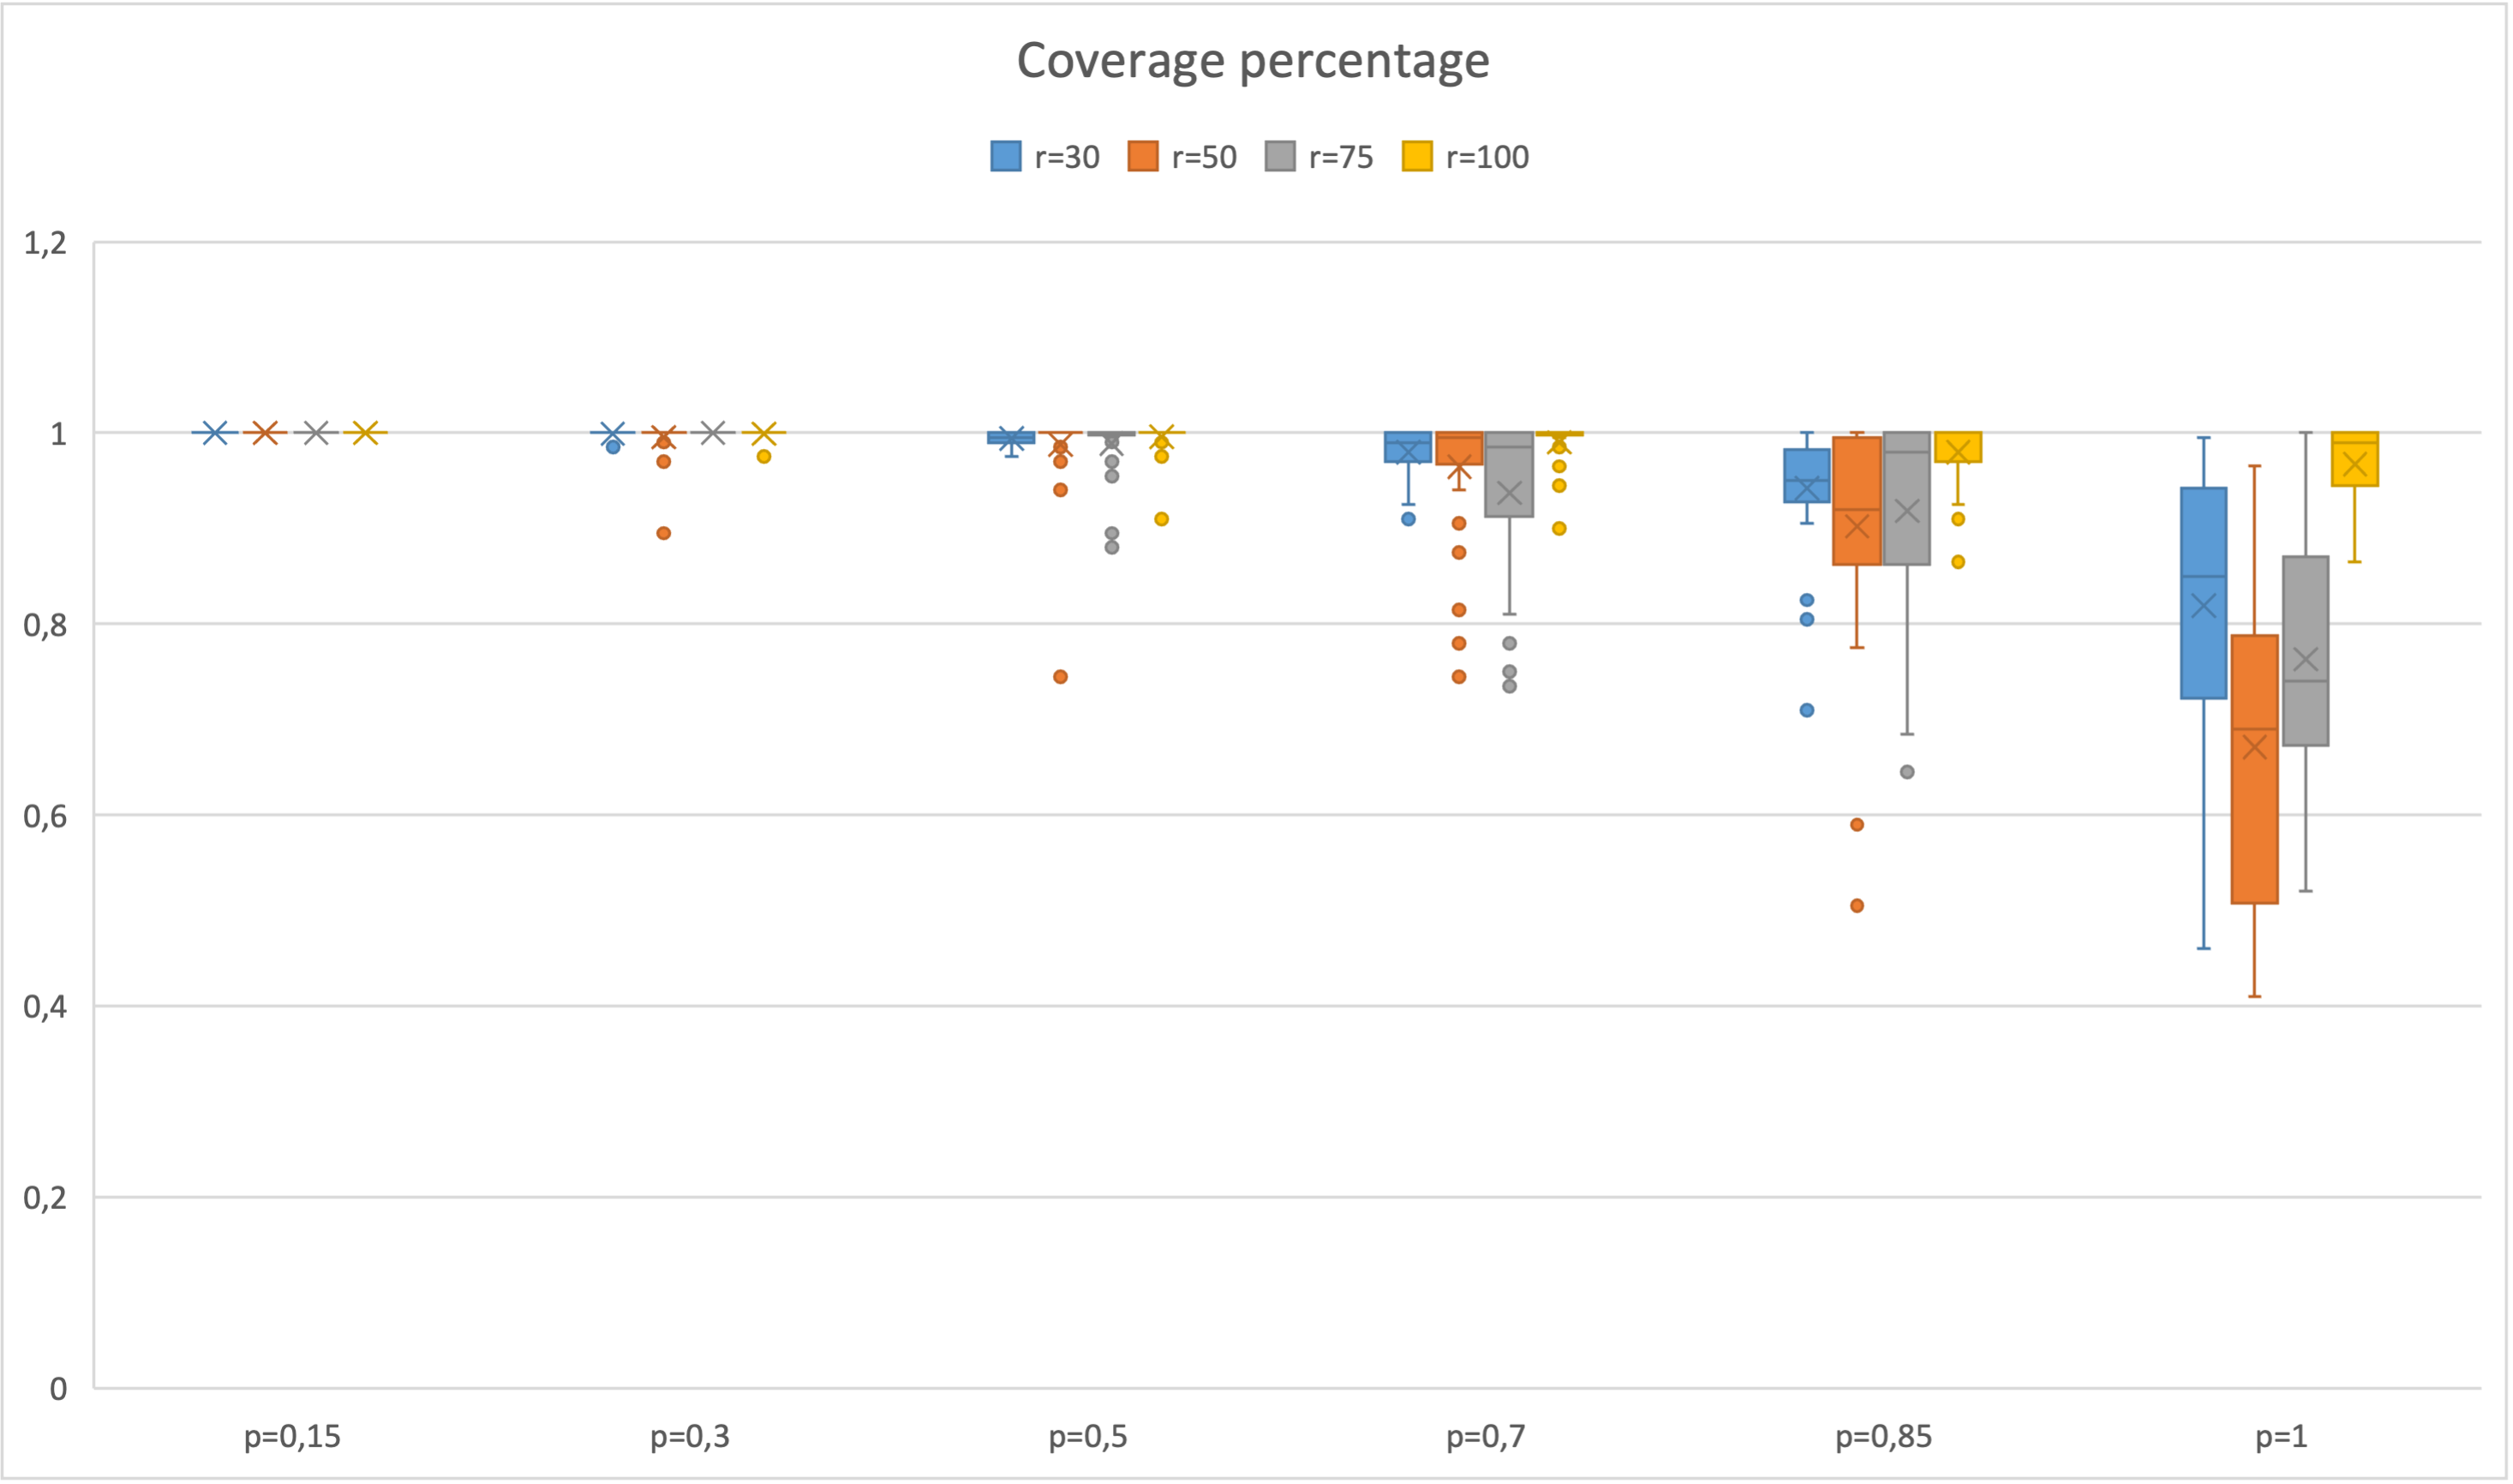
\includegraphics[width=\linewidth]{./images/Rate200Boxplot.png}
  \caption{200 Nodes}\label{fig:awesome_image2}
\endminipage
\end{figure}



\subsection{Coverage time}
\begin{figure}[H]
\minipage{0.50\linewidth}
  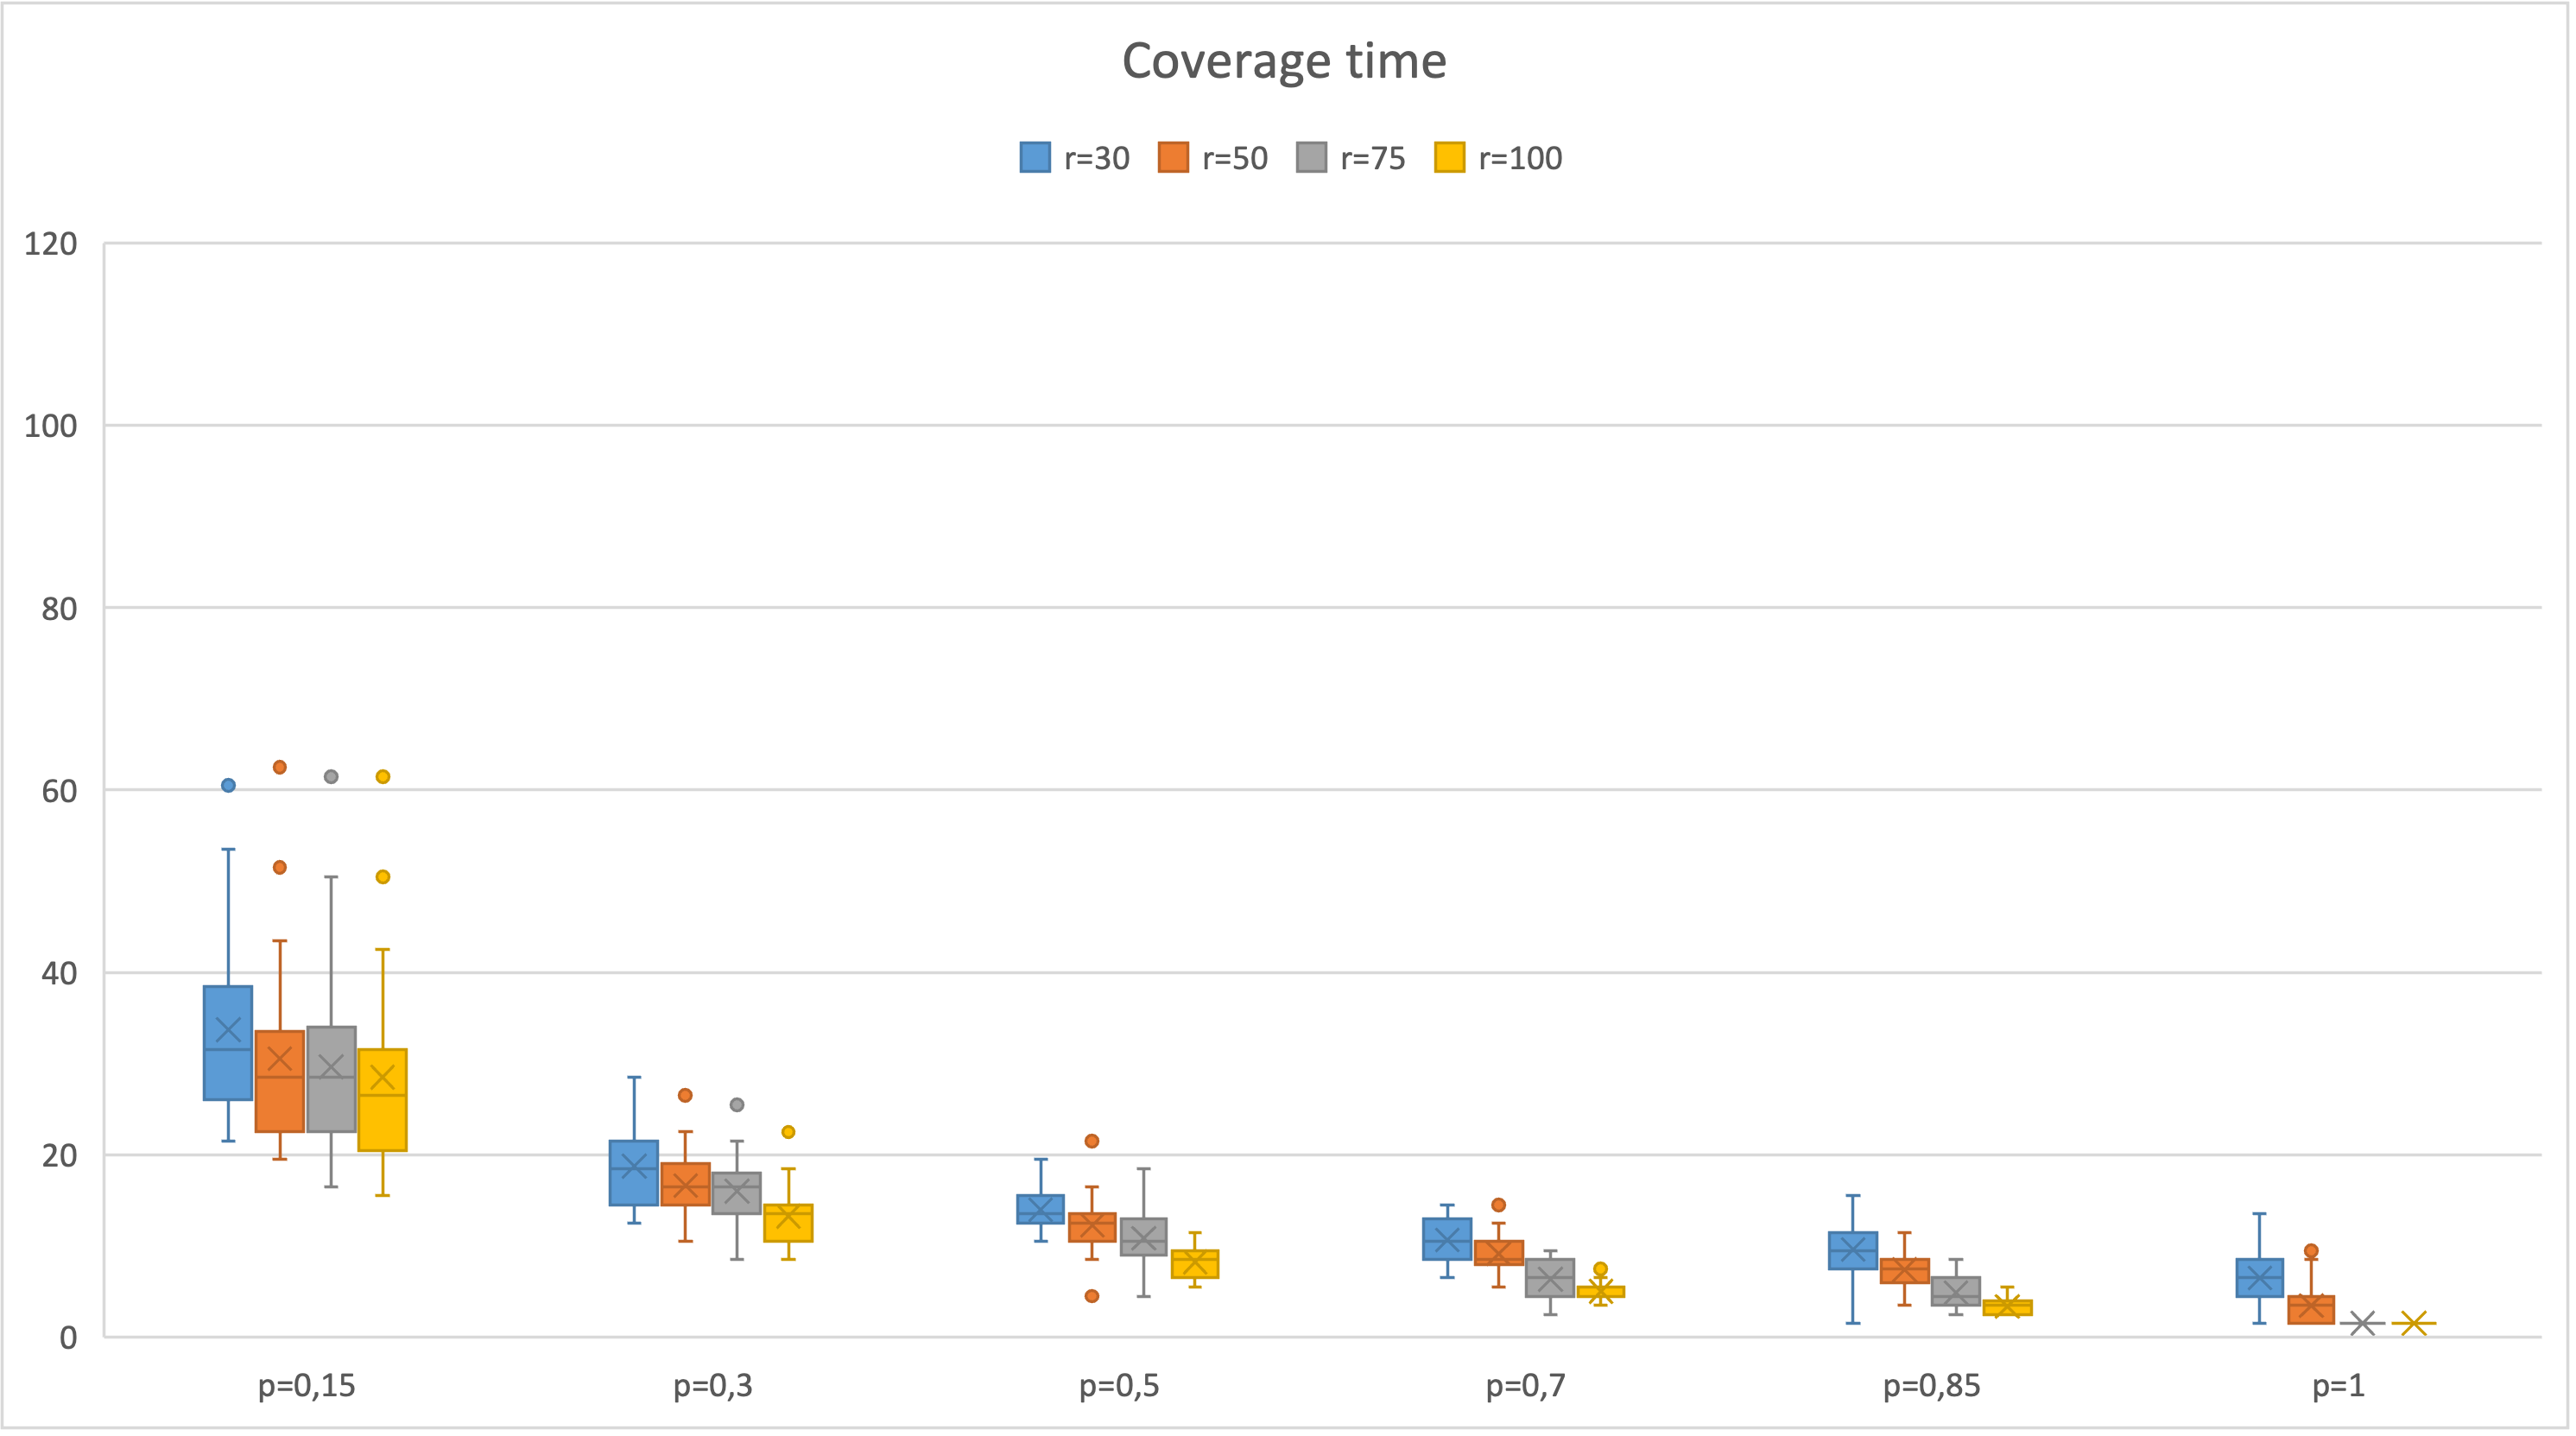
\includegraphics[width=\linewidth]{./images/Time50Boxplot.png}
  \caption{50 Nodes}\label{fig:awesome_image1}
\endminipage\hfill
\minipage{0.50\linewidth}
  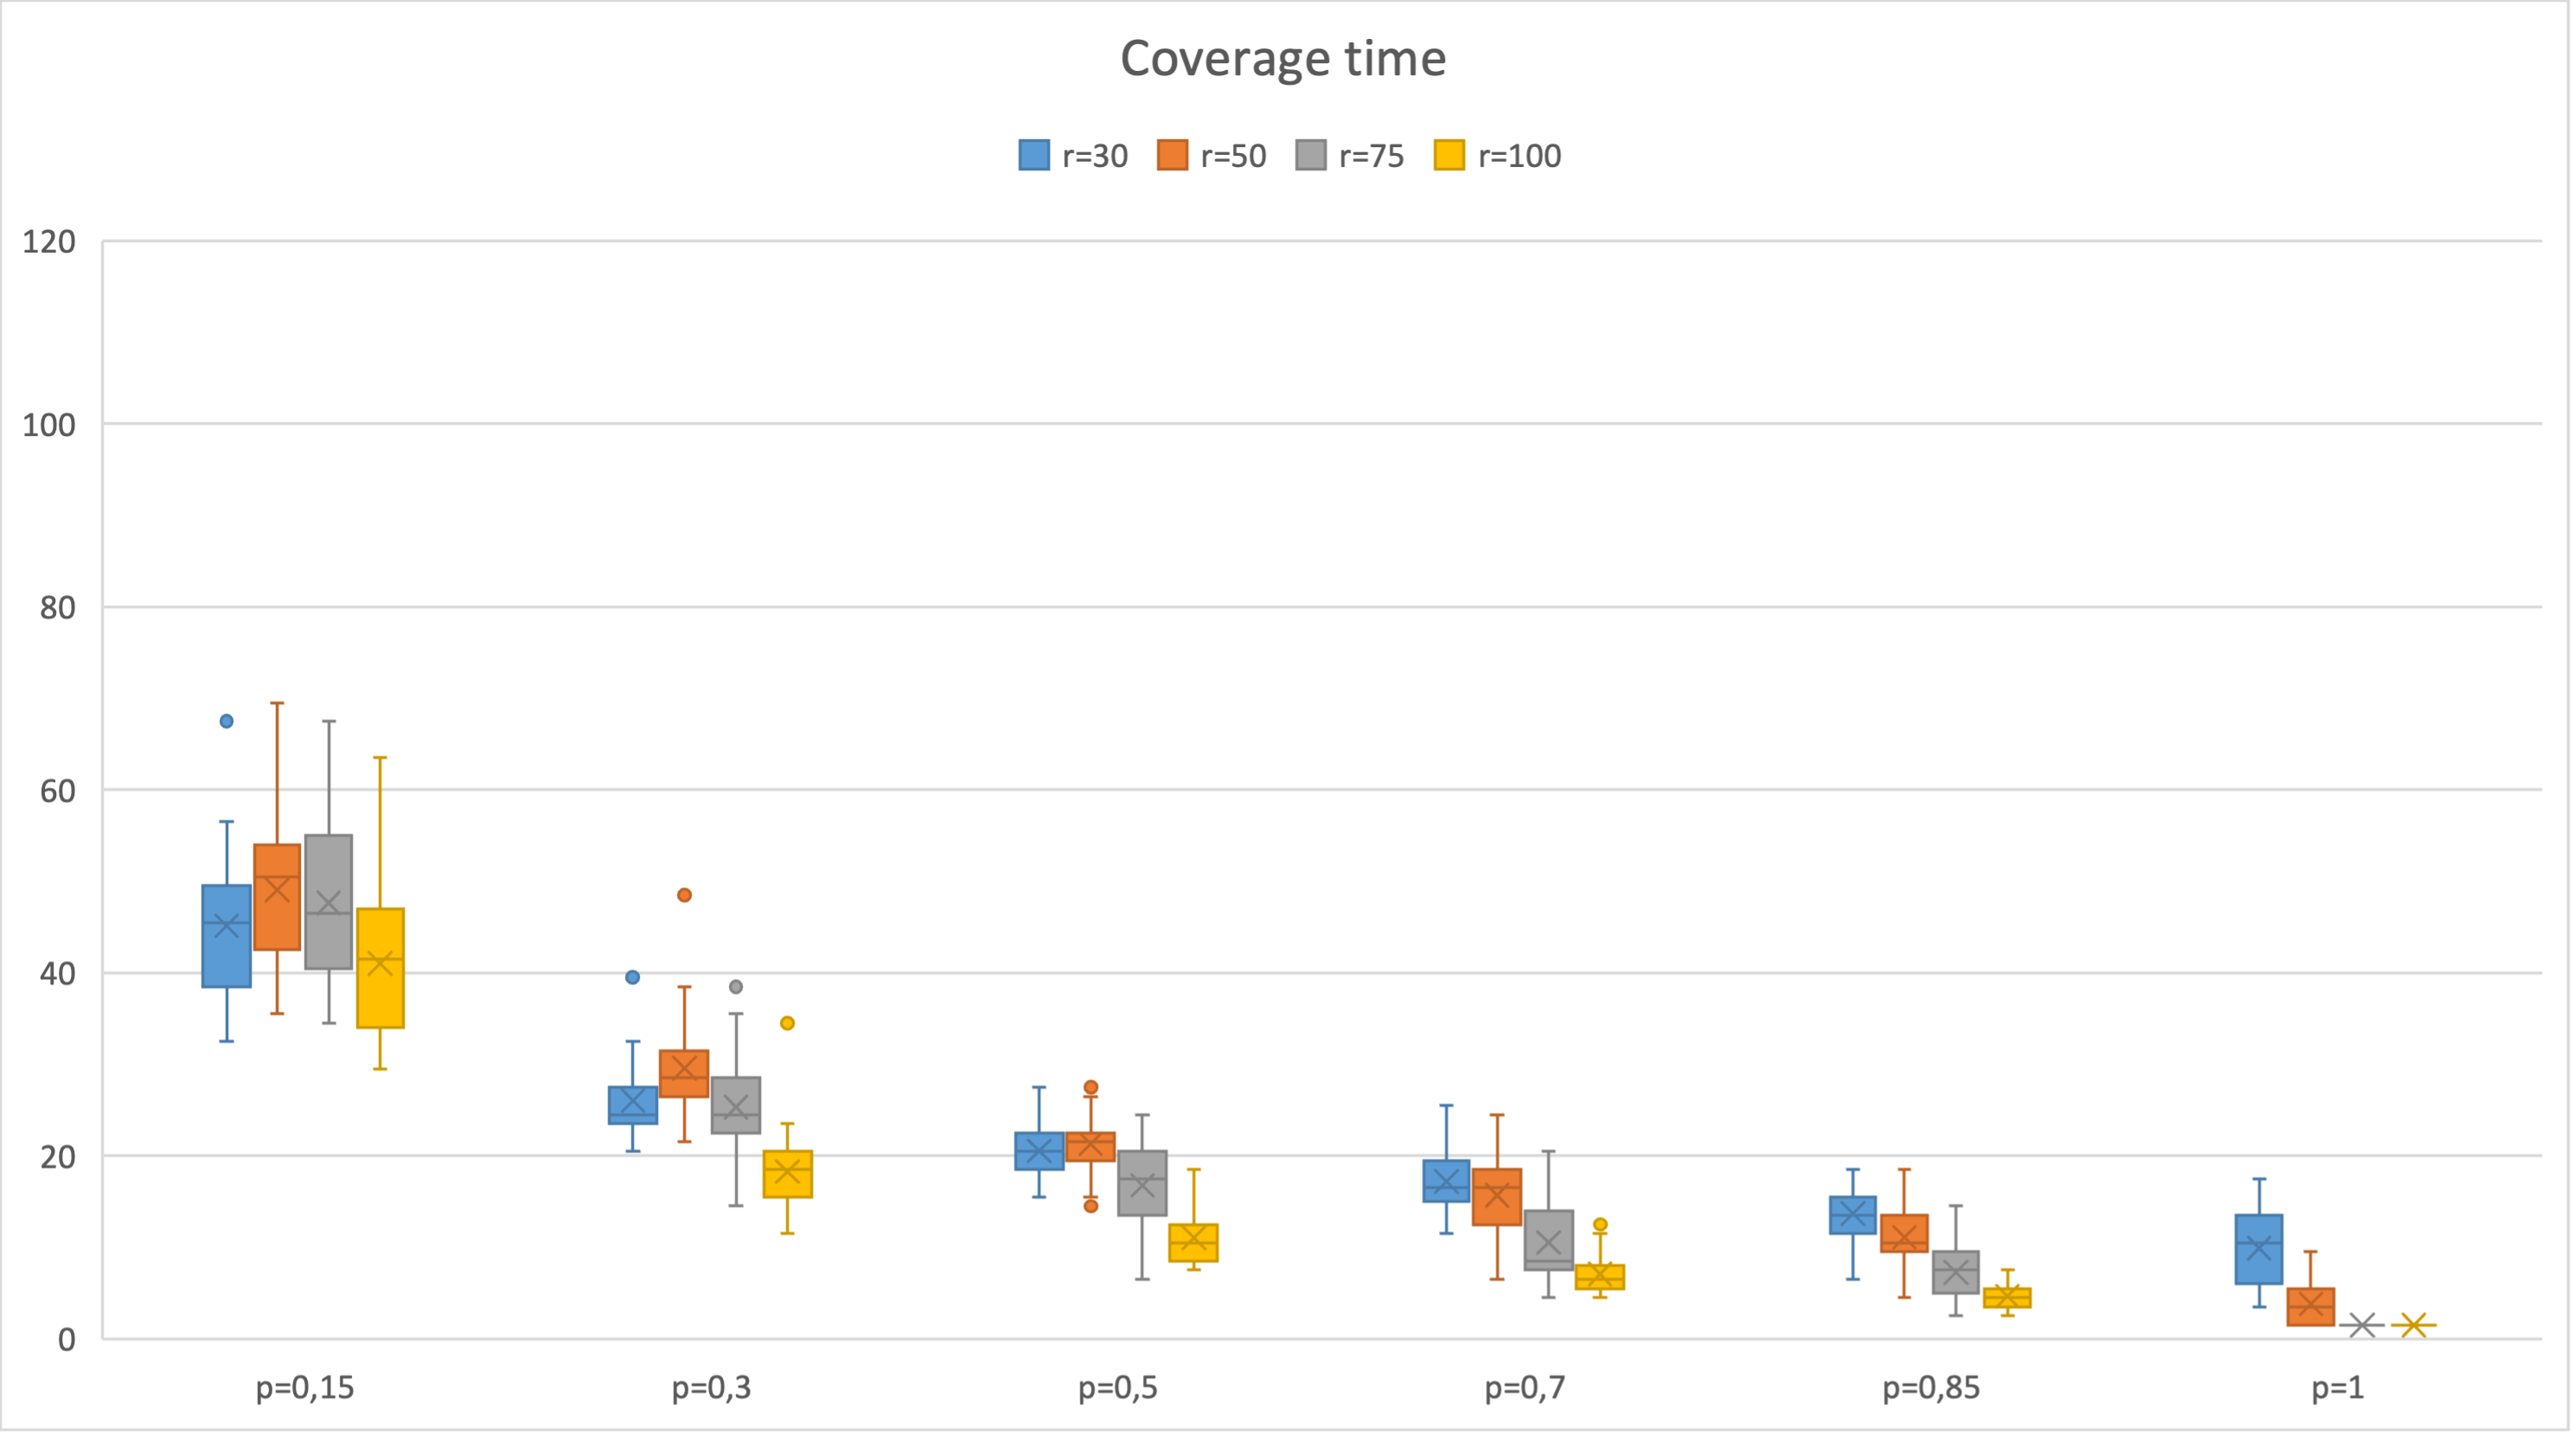
\includegraphics[width=\linewidth]{./images/Time200BoxplotScaled.png}
  \caption{200 Nodes}\label{fig:awesome_image2}
\endminipage
\end{figure}

\begin{figure}[H]
\minipage{0.50\linewidth}
  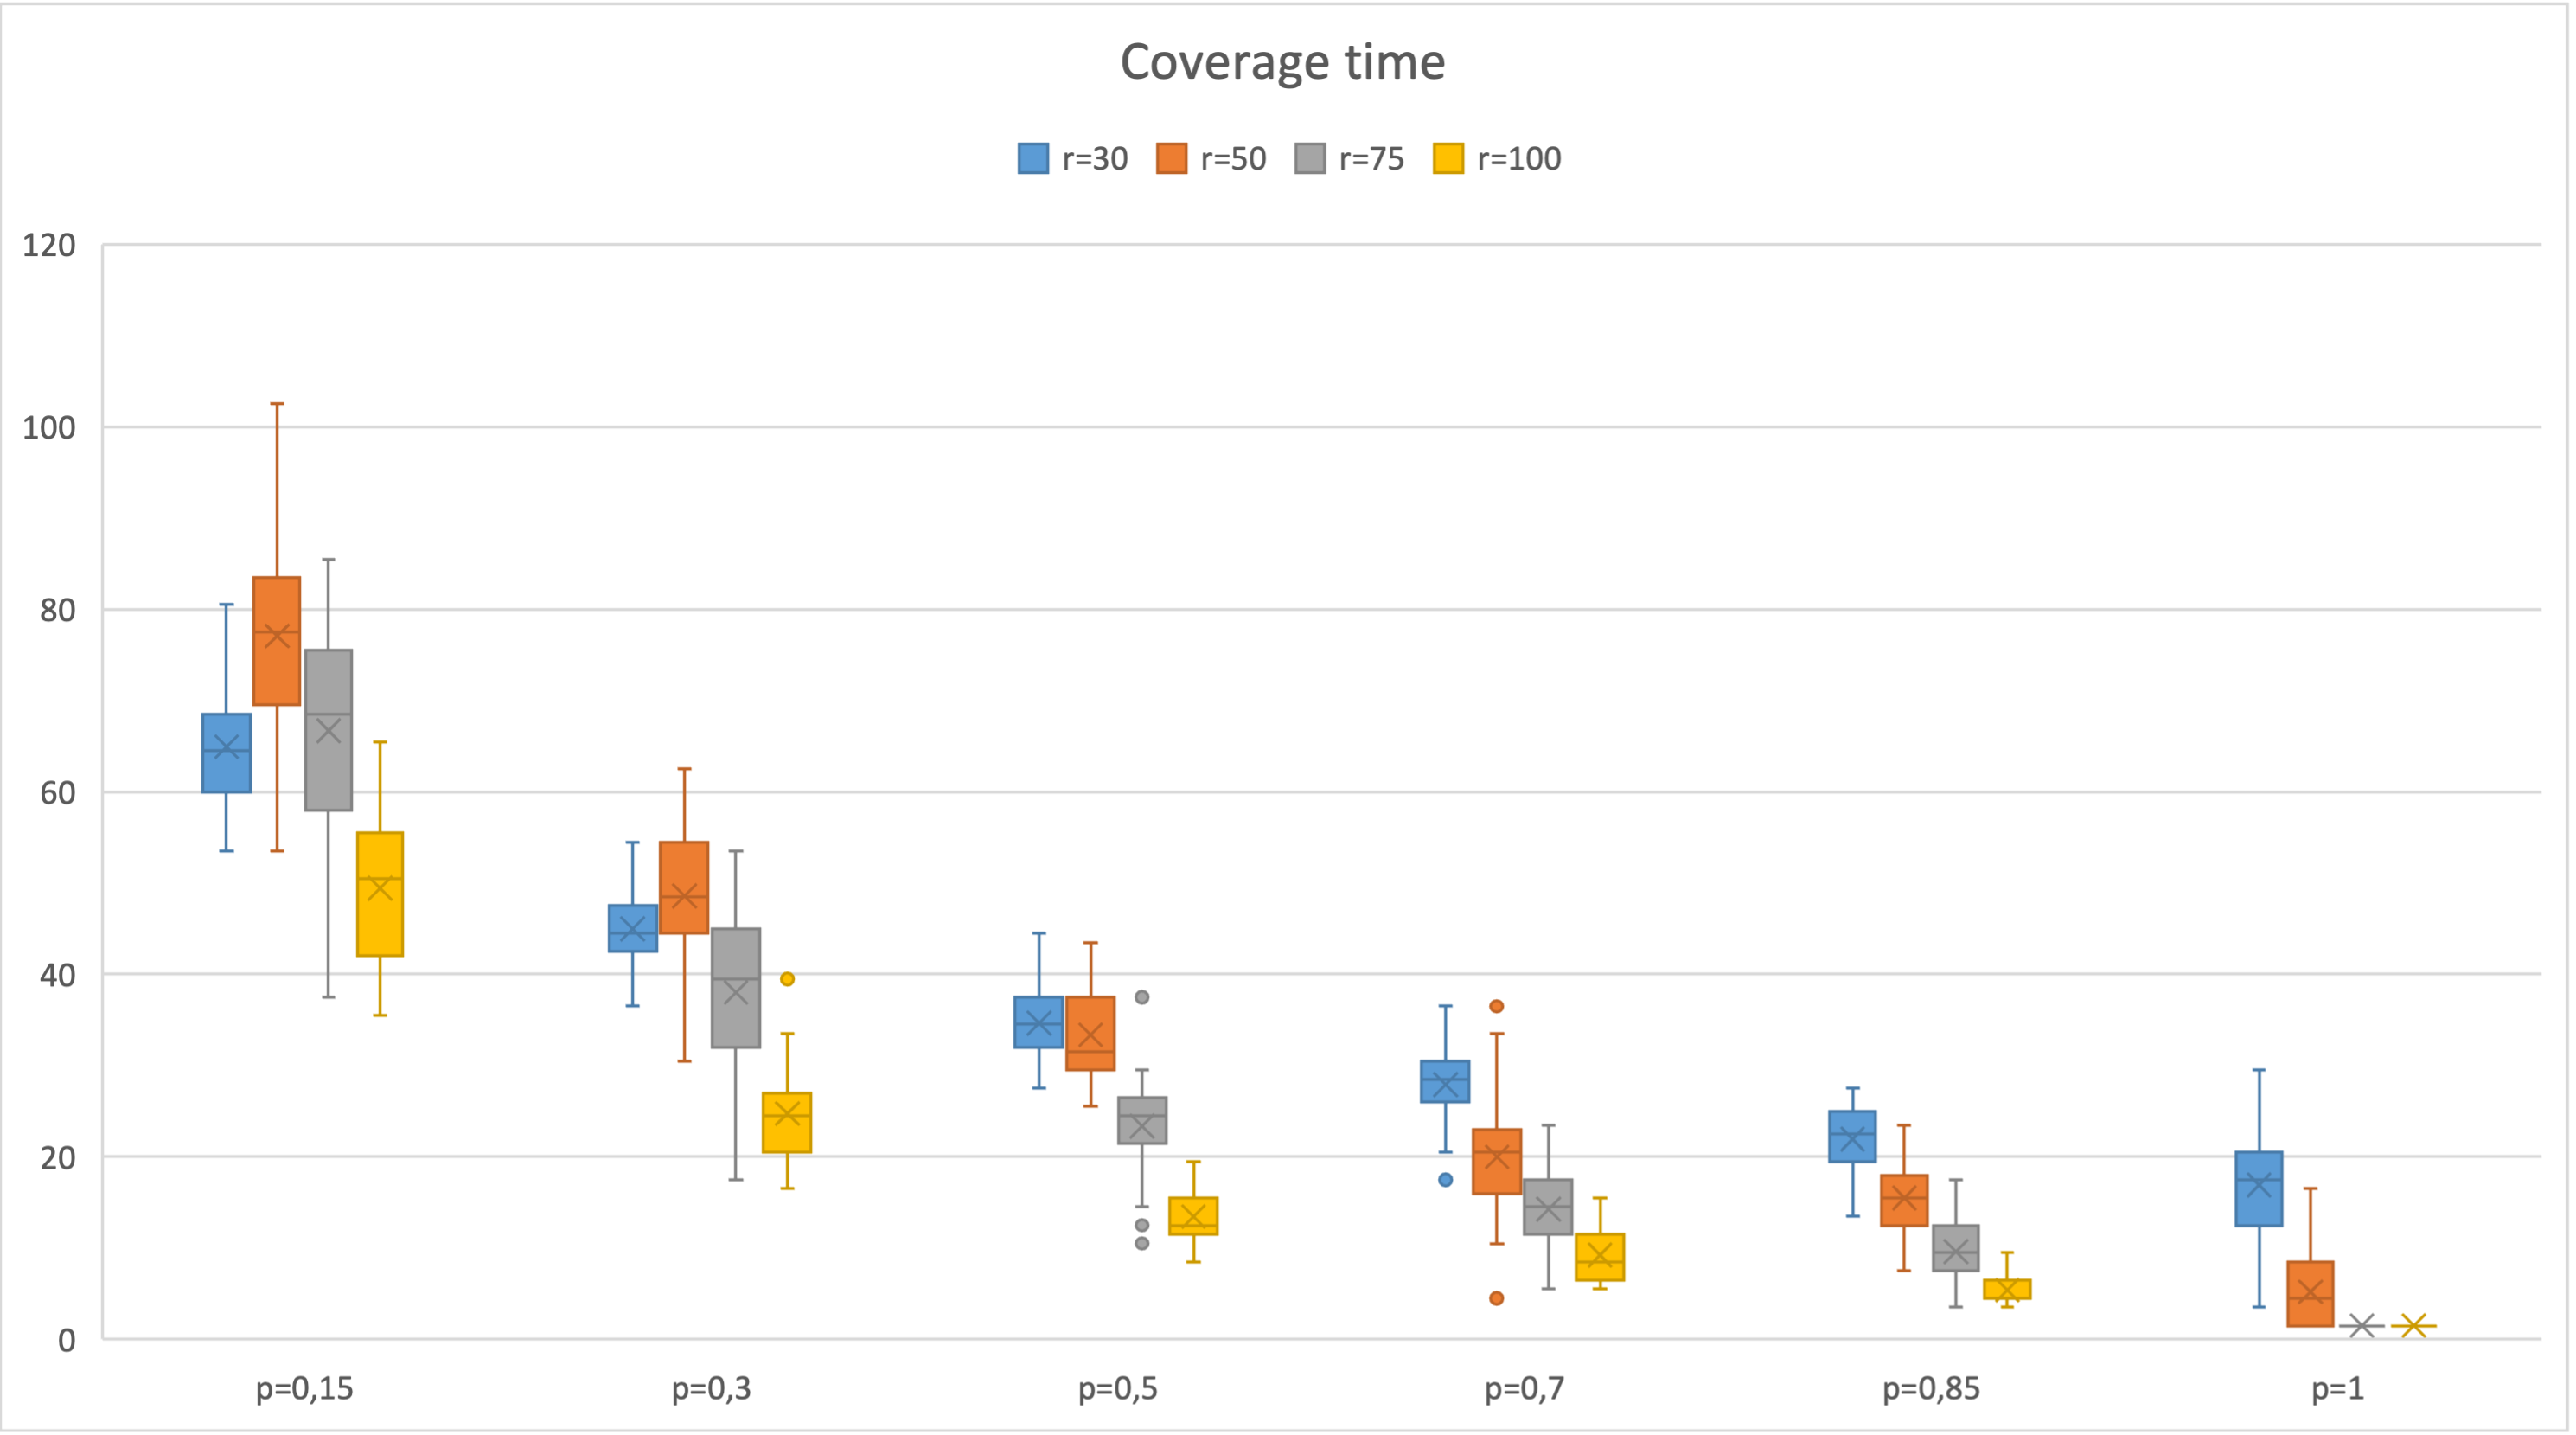
\includegraphics[width=\linewidth]{./images/Time700Boxplot.png}
  \caption{700 Nodes}\label{fig:awesome_image1}
\endminipage\hfill
\minipage{0.50\linewidth}
  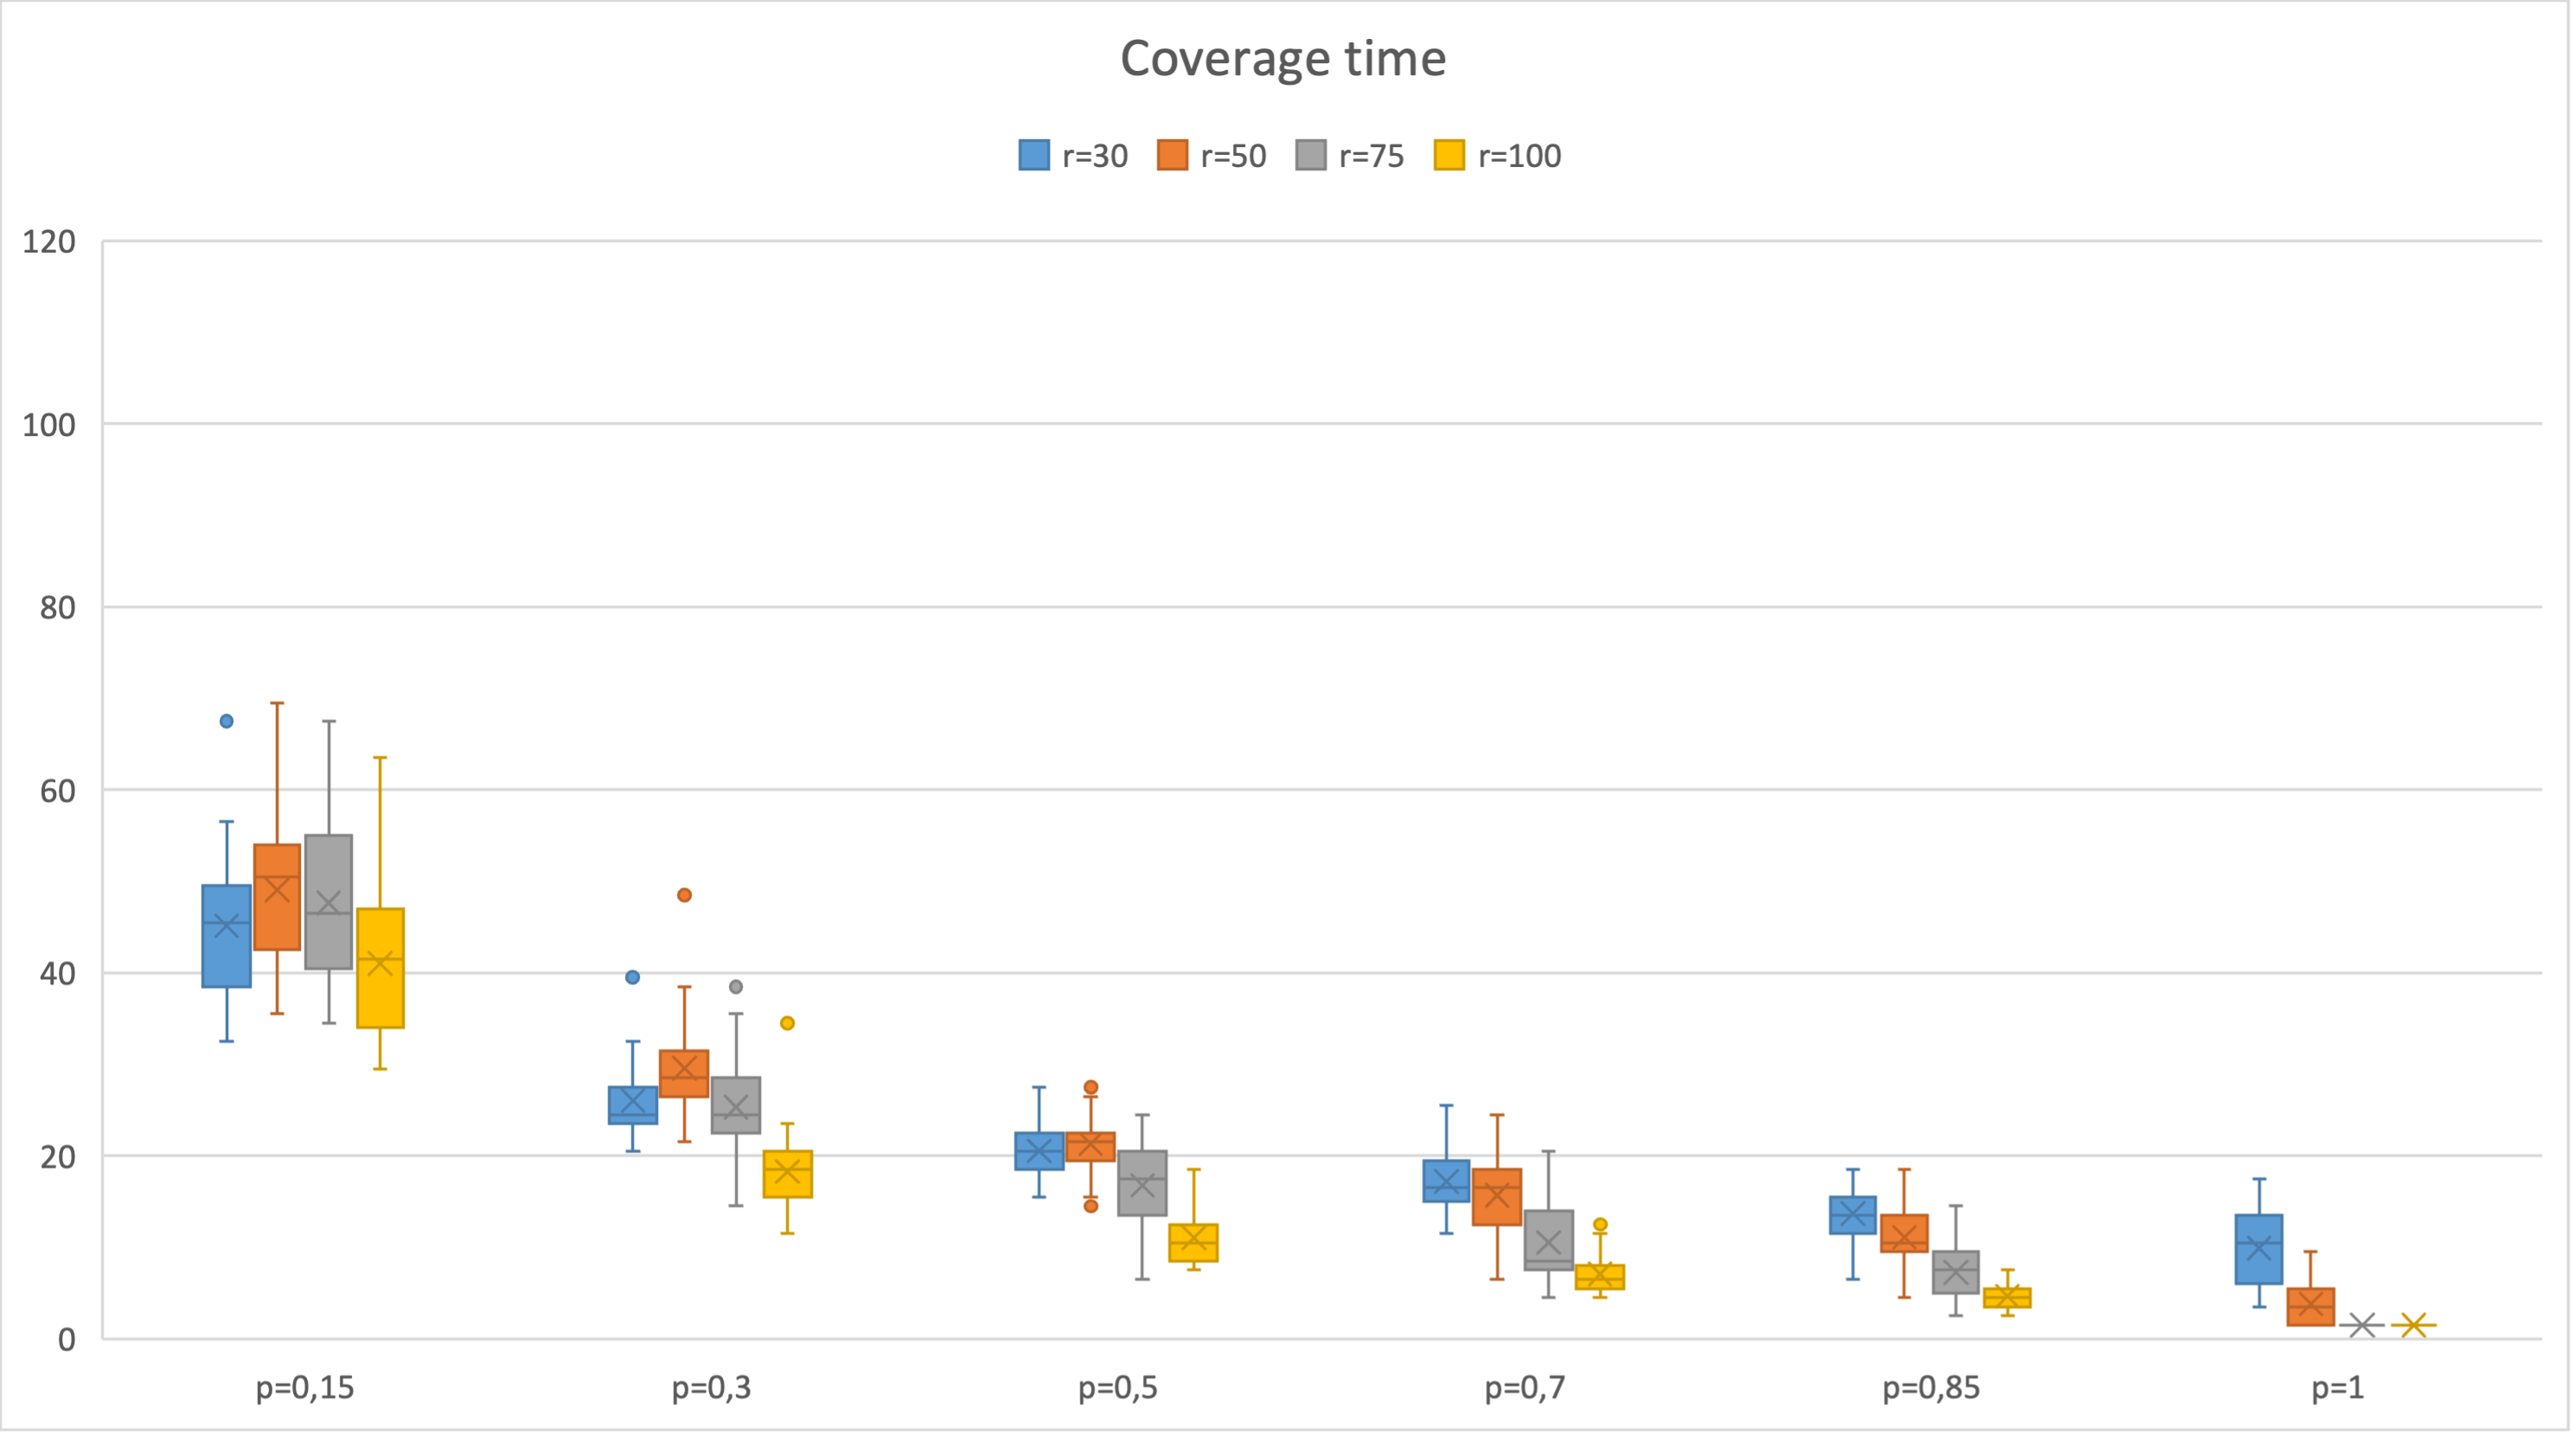
\includegraphics[width=\linewidth]{./images/Time200BoxplotScaled.png}
  \caption{200 Nodes}\label{fig:awesome_image2}
\endminipage
\end{figure}

\subsection{Collision rate}
\begin{figure}[H]
\minipage{0.50\linewidth}
  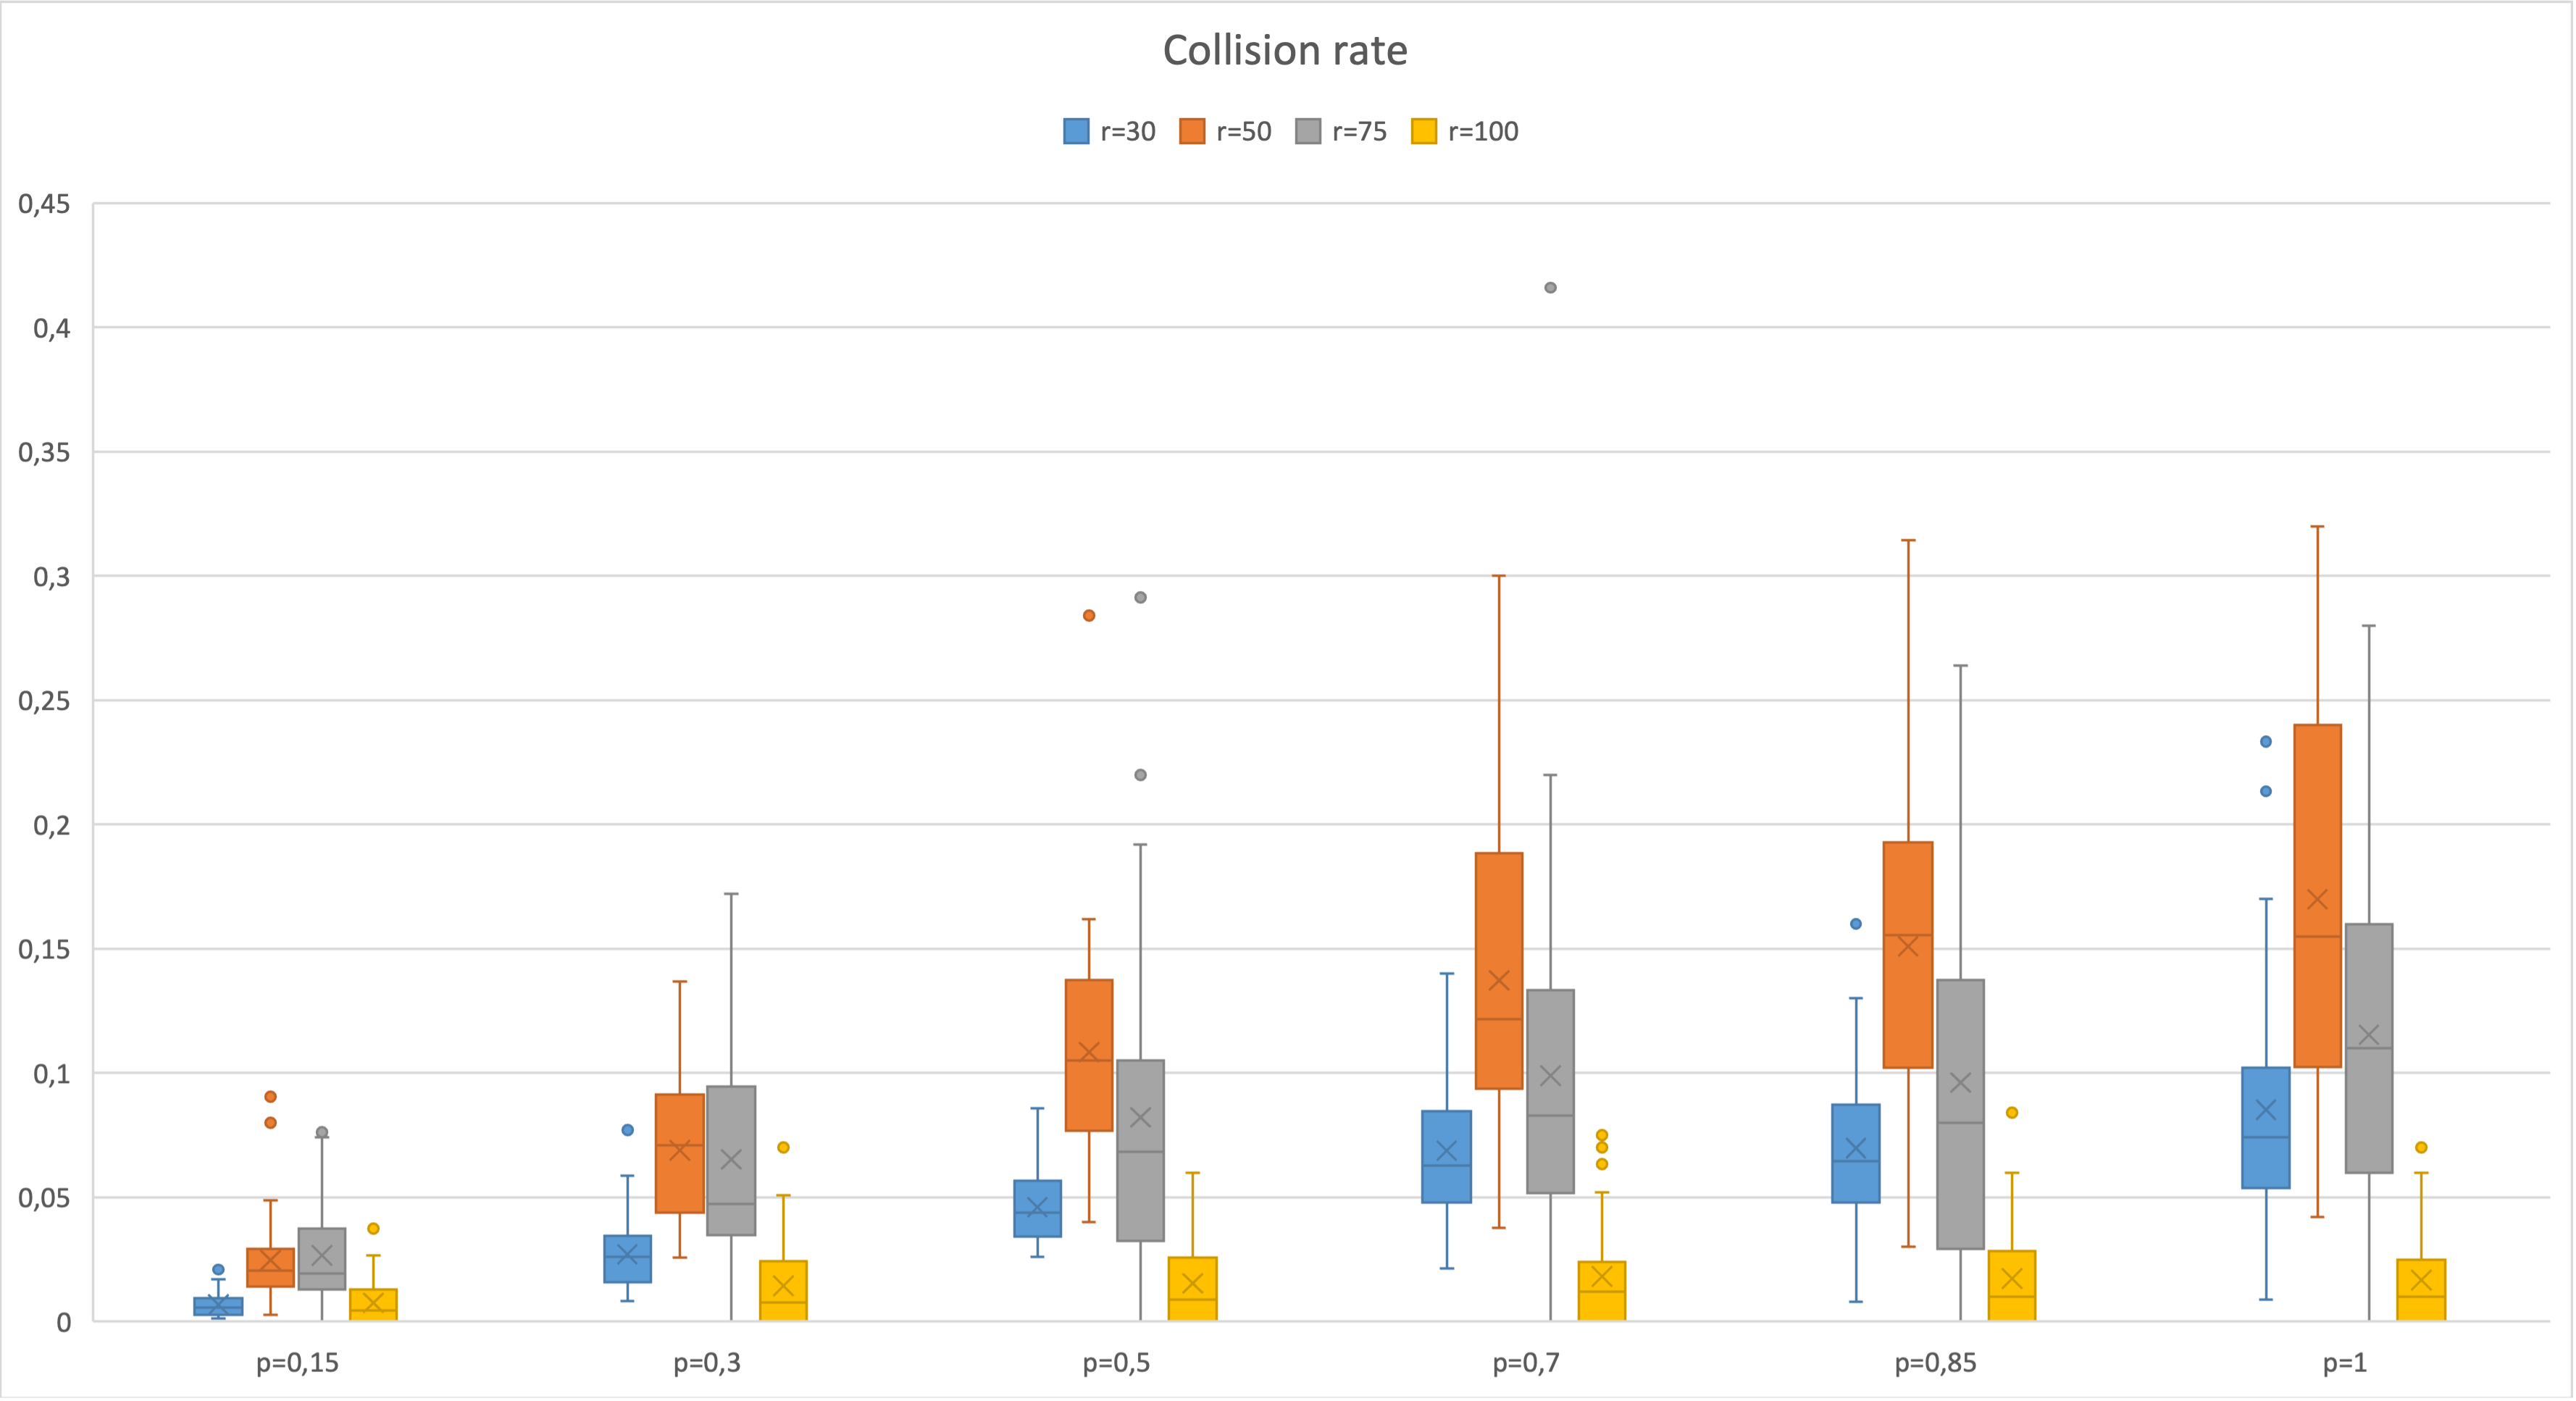
\includegraphics[width=\linewidth]{./images/Collision50Boxplot.png}
  \caption{50 Nodes}\label{fig:awesome_image1}
\endminipage\hfill
\minipage{0.50\linewidth}
  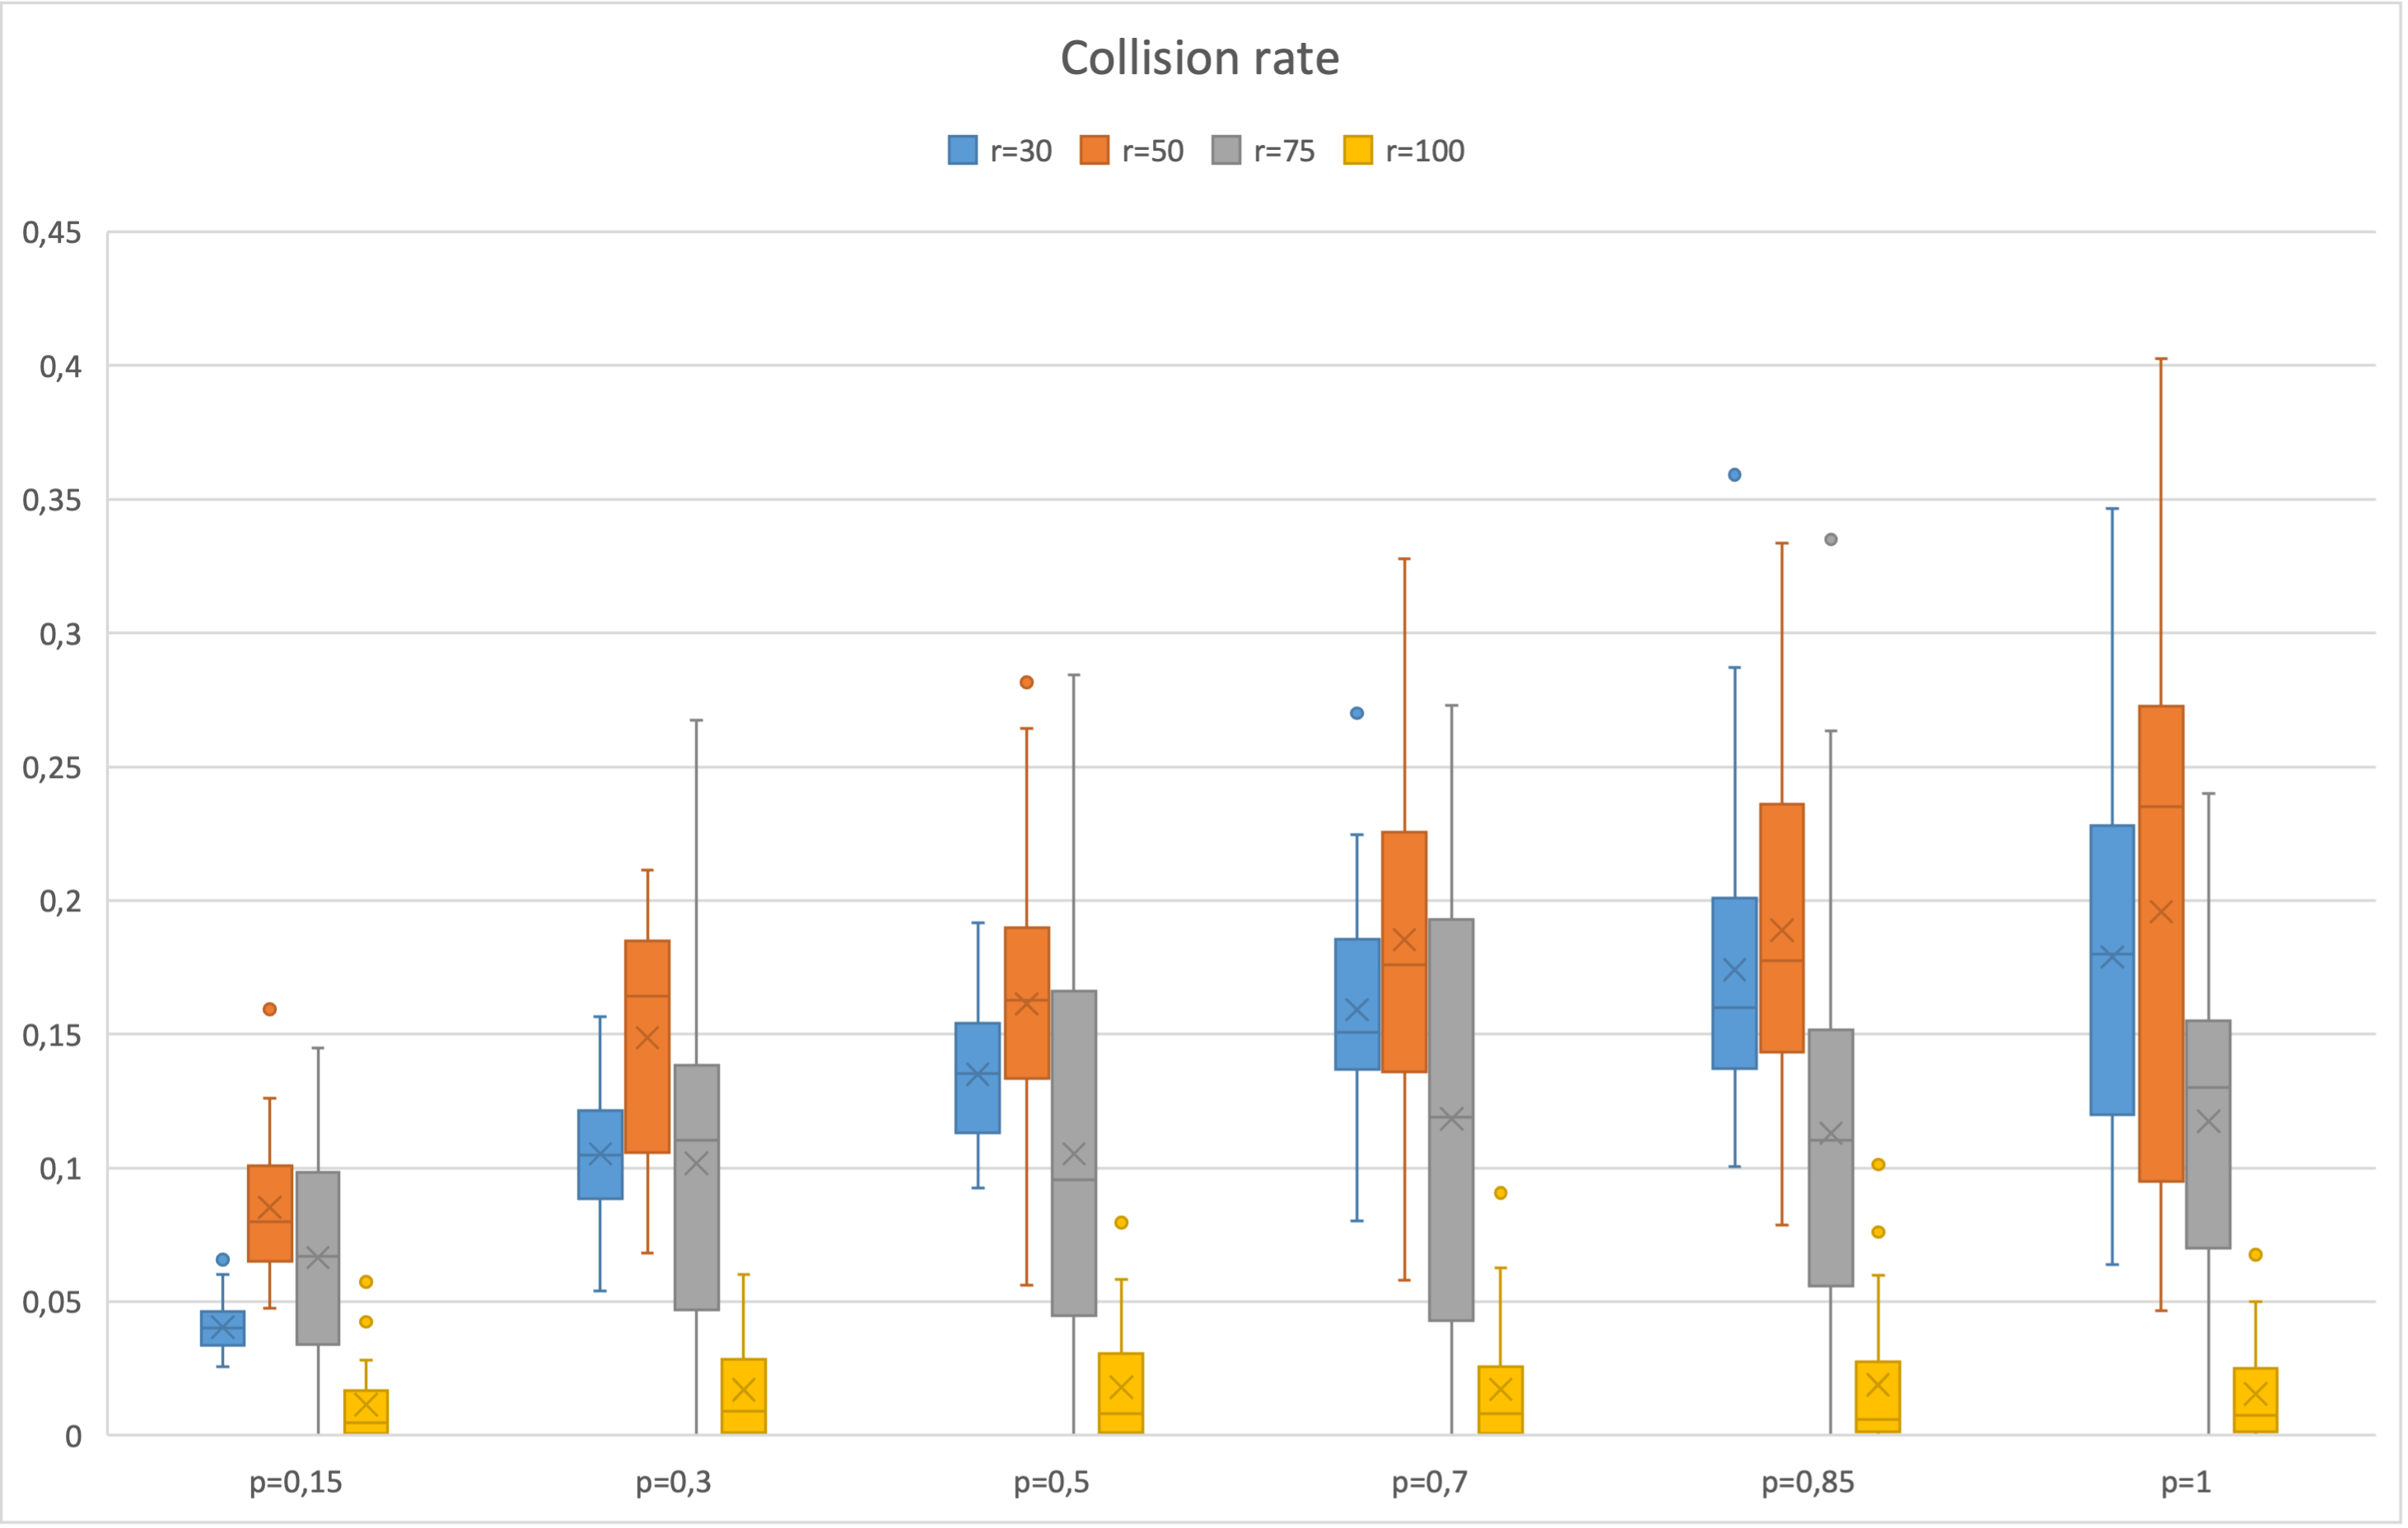
\includegraphics[width=\linewidth]{./images/Collision200Boxplot.png}
  \caption{200 Nodes}\label{fig:awesome_image2}
\endminipage
\end{figure}

\begin{figure}[H]
\minipage{0.50\linewidth}
  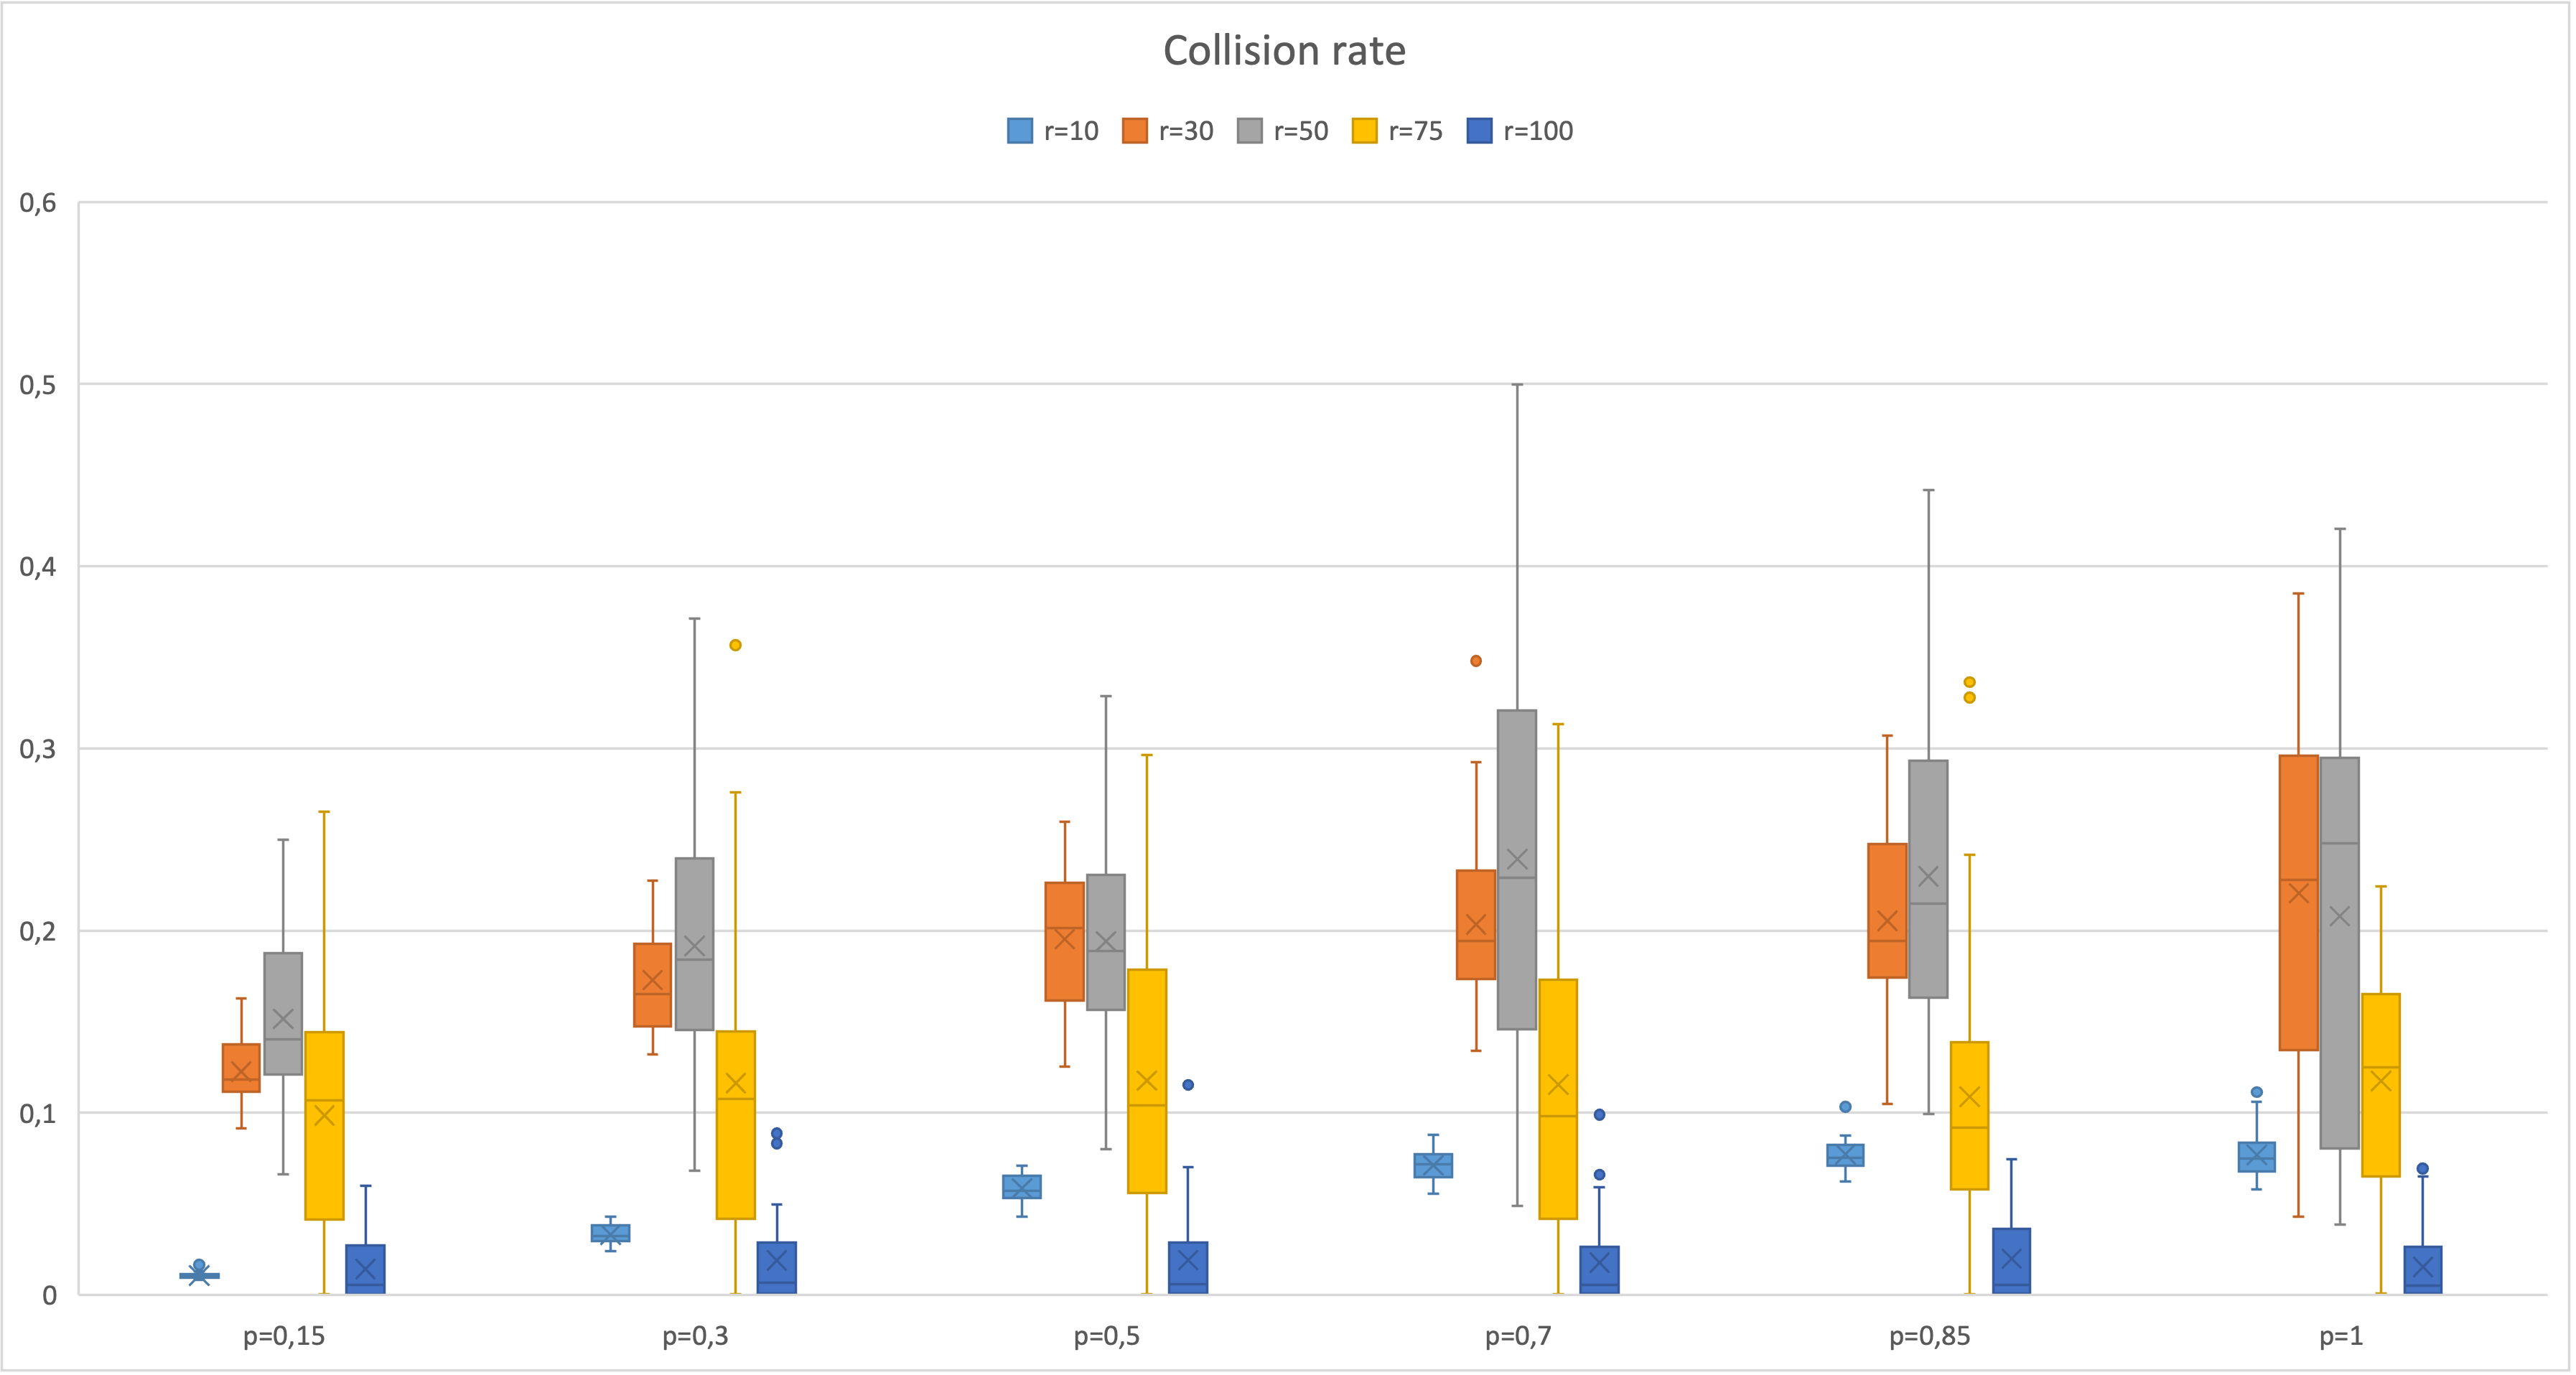
\includegraphics[width=\linewidth]{./images/Collision700Boxplot.png}
  \caption{700 Nodes}\label{fig:awesome_image1}
\endminipage\hfill
\minipage{0.50\linewidth}
  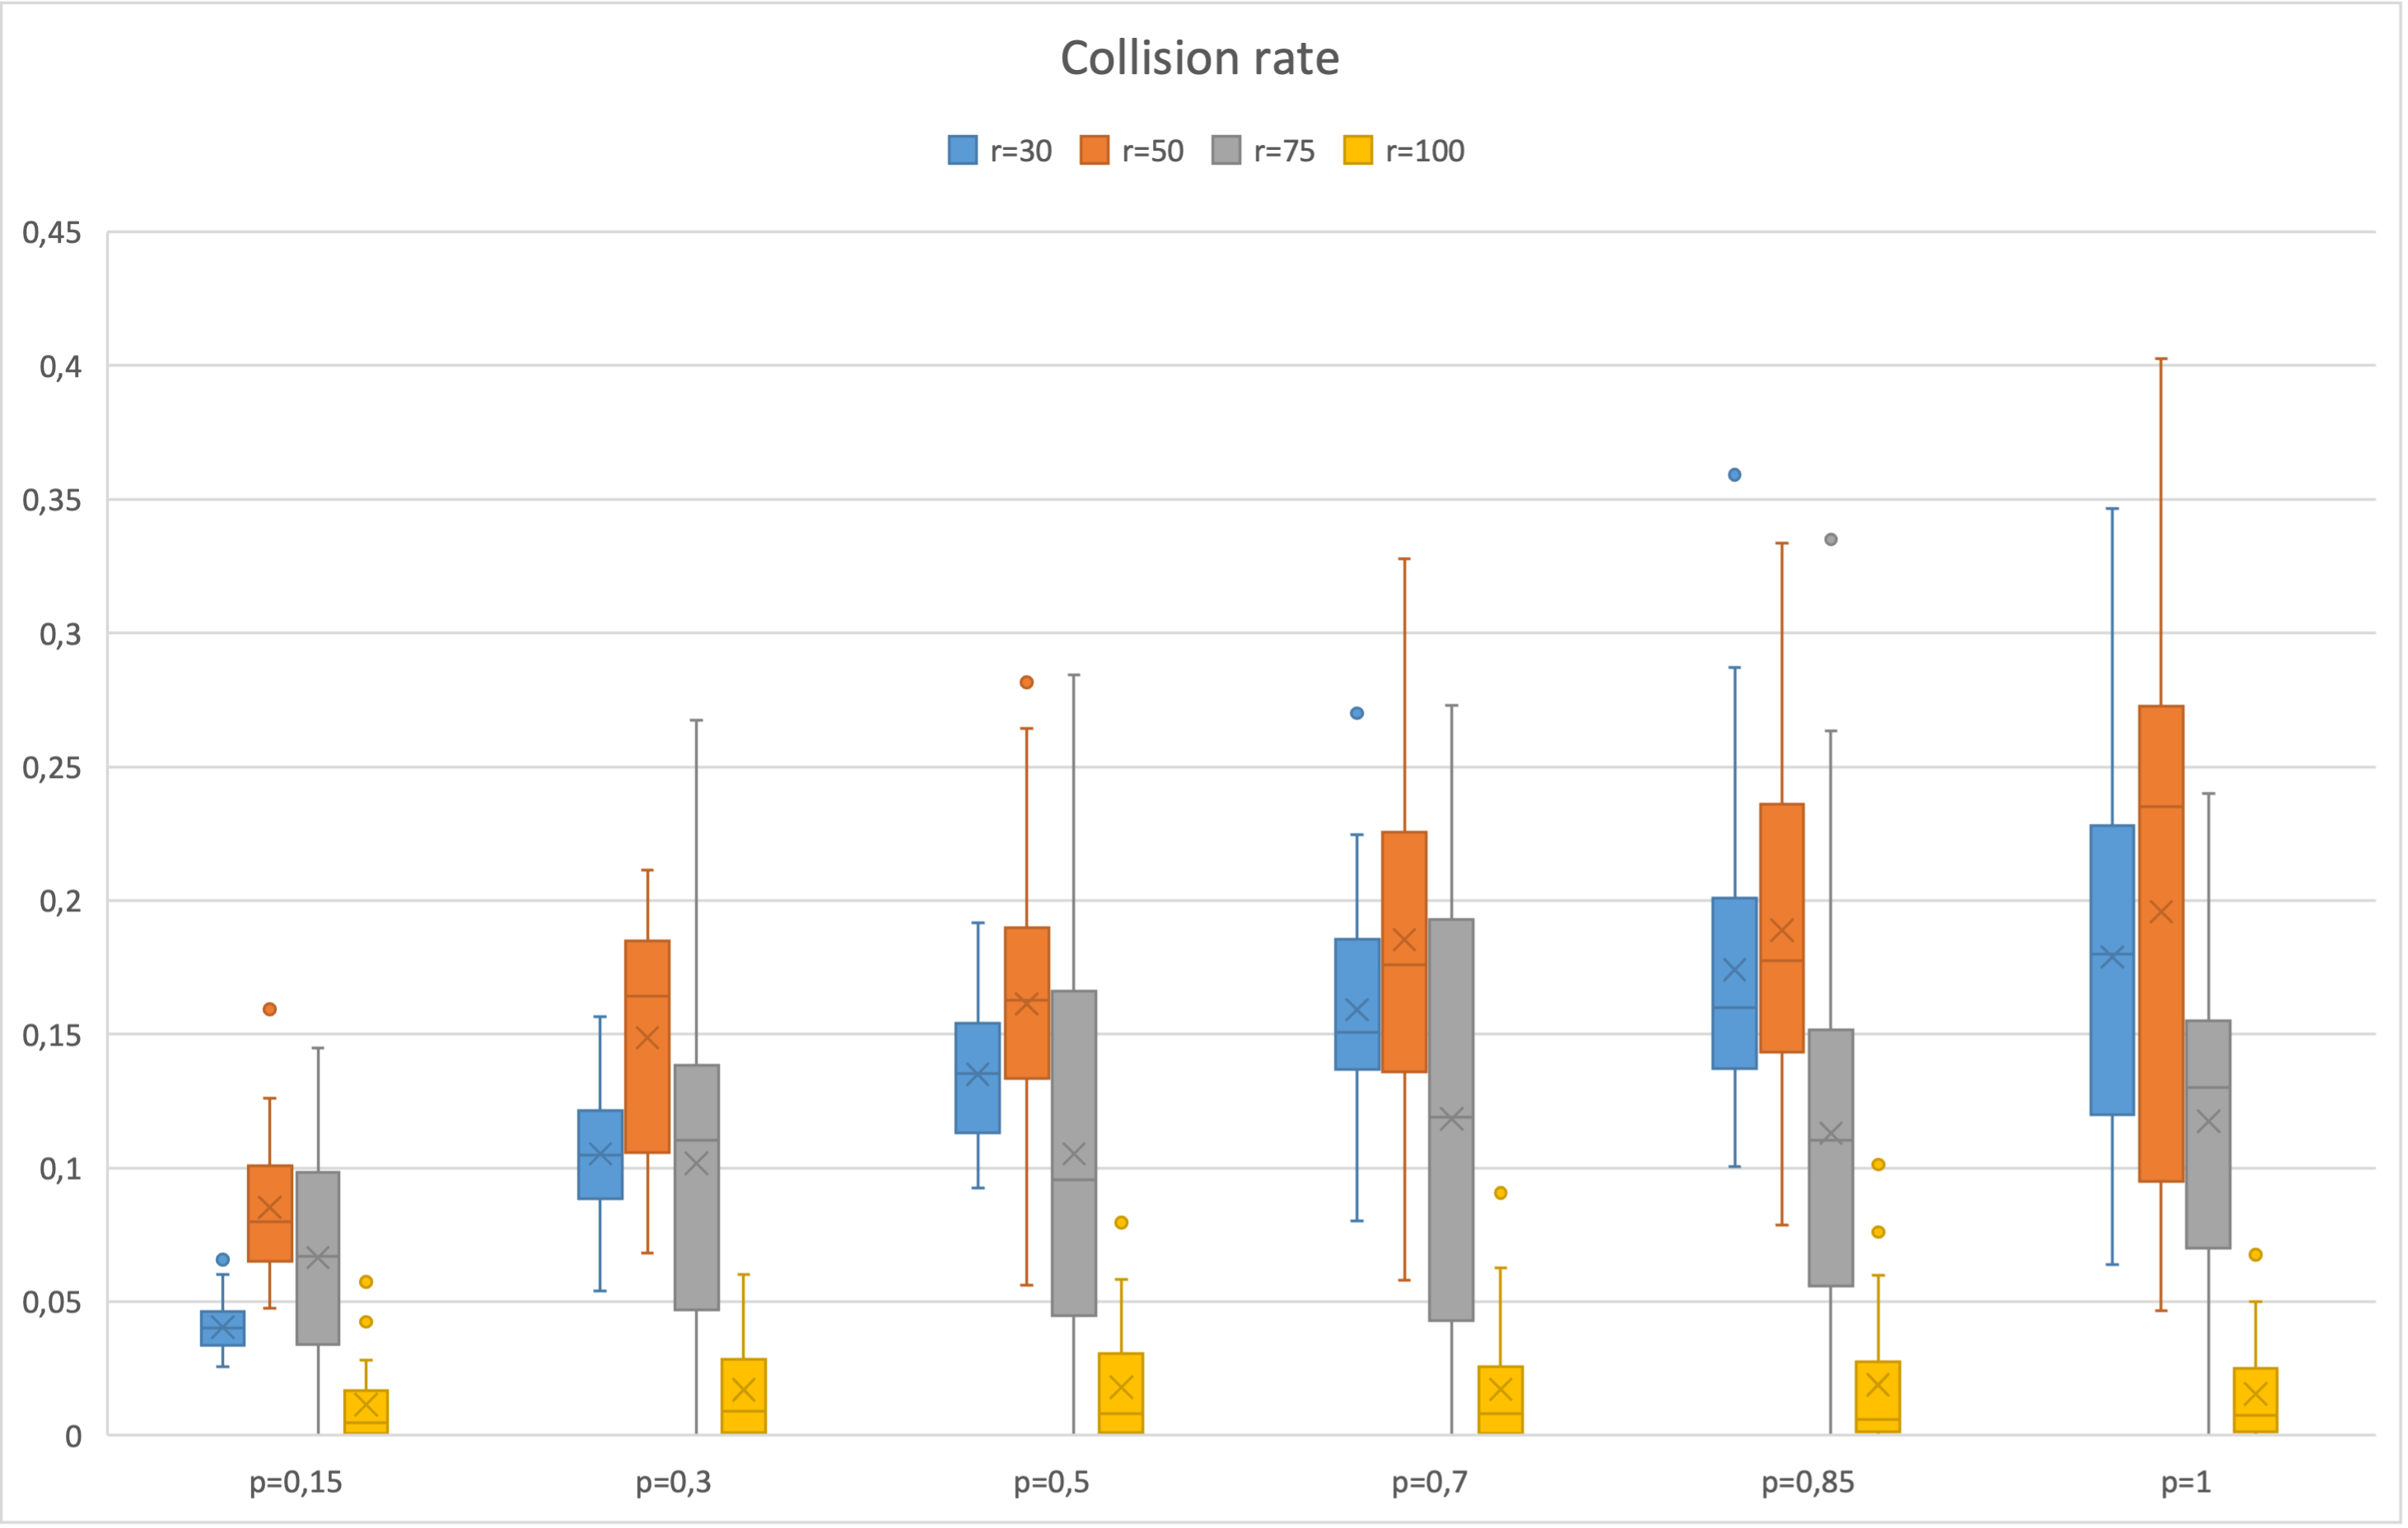
\includegraphics[width=\linewidth]{./images/Collision200Boxplot.png}
  \caption{200 Nodes}\label{fig:awesome_image2}
\endminipage
\end{figure}

By varying the number of nodes, the visible trends for the case of 200 nodes seem to be confirmed (insert quote). As regards the coverage time at low probabilities, an increase is noted, as expected, as the number of nodes increases.